\chapter{Simulation, Reconstruction, and Event Reduction}
\label{chap:Simulations}

As a crucial part of the oscillation analysis, an accurate prediction of the expected neutrino spectrum at the far detector is required. This includes modeling the flux generation, neutrino interactions, and detector effects. All of the simulation packages required to do this are briefly described in \autoref{sec:Simulations_Simulation}. The reconstruction of neutrino events in the far detector, including the \texttt{fiTQun} algorithm, is documented in \autoref{sec:Simulation_Reconstruction}. This also includes data quality checks of the SK-V data which the author performed for the T2K oscillation analysis presented at the Neutrino 2020 conference \cite{Dunne2020-uf}. Finally, \autoref{sec:Simulations_Reduction} describes the steps taken in the SK detector to trigger on events of interest whilst removing the comparatively large rate of cosmic ray muon events.

\section{Simulation}
\label{sec:Simulations_Simulation}

In order to generate a Monte Carlo prediction of the expected event rate at the far detector, all the processes in the beam and atmospheric fluxes, neutrino interaction, and detector need to be modeled. %Each of these parts is individually modeled and each of them is detailed below.

\subsection{Neutrino Flux}

The beamline simulation consists of three distinct parts: the initial hadron interaction modeled by FLUKA \cite{fluka2011}, the target station geometry and particle tracking performed by JNUBEAM, \cite{geant3, PhysRevD.87.012001} and any hadronic re-interactions simulated by GCALOR \cite{gcalor}. The primary hadronic interactions are \quickmath{O(10)\text{GeV}}, where FLUKA matches external cross-section data better than GCALOR \cite{t2k_tn_flux}. However, FLUKA is not very adaptable so a small simulation is built to model the interactions in the target and the output is then passed to JNUBEAM and GCALOR for propagation. The hadronic interactions are tuned to data from the NA61/SHINE \cite{Abgrall_2011, Abgrall_2012, NA61_pions_rep} and HARP \cite{harp} experiments. The tuning is done by reweighting the FLUKA and GCALOR predictions to match the external data multiplicity and cross-section measurements, based on final state particle kinematics \cite{t2k_tn_flux}. The culmination of this simulation package generates the predicted flux for neutrino and antineutrino beam modes which are illustrated in \autoref{fig:T2KSKExp_T2K_NuFluxPerMode}.

The atmospheric neutrino flux is simulated by the HKKM model \cite{Honda_2007, Honda:2011}. The primary cosmic ray flux is tuned to AMS \cite{Blau2002} and BESS \cite{Haino2004} data assuming the US-standard atmosphere `76 \cite{USStandardAtm} density profile and includes geomagnetic field effects. The primary cosmic rays interact to generate pions and muons. The interaction of these secondary particles to generate neutrinos is handled by DPMJET-III \cite{Roesler2001} for energies above \quickmath{32\text{GeV}} and JAM \cite{Niita2006, Honda:2011} for energies below that value \cite{Gaisser2002-gl}. These hadronic interactions are tuned to BESS and L3 data \cite{Sanuki_2002, Achard_2004} using the same methodology as the tuning of the beamline simulation. The energy and cosine zenith predictions of \quickmath{\nu_{e}, \bar{\nu}_{e}, \nu_{\mu}, \bar{\nu}_{\mu}} flux are given in \autoref{fig:NeutrinoOscillationPhysics_AtmosphericNeutrinoFlux} and \autoref{fig:NeutrinoOscillationPhysics_NuFluxZenithAngleDep}, respectively. The flux is approximately symmetrical and peaked around the horizon (\quickmath{\cos(\theta_{Z}) = 0.0}). This is because horizontally-going pions and kaons can travel further than their vertically-going counterparts resulting in a larger probability of decaying to neutrinos. The symmetry is broken in lower-energy neutrinos due to geomagnetic effects, which modify the track of the primary cosmic rays. Updates to the HKKM model are currently ongoing \cite{Sato2022-ss}.

\subsection{Neutrino Interaction}

Once a flux prediction has been made for all three detectors, NEUT 5.4.0 \cite{Hayato2021, neut} models the interactions of the neutrinos in the detectors. For the purposes of this analysis, quasi-elastic (QE), meson exchange (MEC), single meson production (PROD), coherent pion production (COH), and deep inelastic scattering (DIS) interactions are simulated. These interaction categories can be further broken down by whether they were propagated via a \quickmath{W^{\pm}} boson in Charged Current (CC) interactions or via a \quickmath{Z^{0}} boson in Neutral Current (NC) interactions. CC interactions have a charged lepton in the final state, which can be flavour-tagged in reconstruction to determine the flavour of the neutrino. In contrast, NC interactions have a neutrino in the final state so no flavour information can be determined from the observables left in the detector after an interaction. This is the reason why neutrinos that interact through NC modes are assumed to not oscillate within this analysis. Both CC and NC interactions are modeled for all the above interaction categories, other than MEC interactions which are only modeled for CC events. 
%As the SK detector is only sensitive to charged particles above Cherenkov threshold, all charged current interactions are simulated whilst only neutral current processes that can produce charged particles (NCDIS, NCCOH, and NCPROD including $\pi^{0}$ production) are modeled. NC MEC interactions can only produce charged particles through secondary re-interactions which is a low cross-section process.

\begin{figure}[h]
  \begin{subfigure}[t]{0.8\textwidth}
    \includegraphics[width=\textwidth, trim={0mm 0mm 0mm 0mm}, clip,page=1]{Figures/Simulations/NEUTCrossSection.pdf}
  \end{subfigure}
  \caption{The NEUT prediction of the \quickmath{\nu_{\mu}}-H2O cross-section overlaid on the T2K \quickmath{\nu_{\mu}} flux. The charged current (black, solid) and neutral current (black, dashed) inclusive, charged current quasi-elastic (blue, solid), charged current 2p2h (blue, dashed), charged current single pion production (pink), and charged current multi--\quickmath{\pi} and DIS (Purple) cross-sections are illustrated. Figure taken from \cite{Hayato2021}.}
  \label{fig:Simulations_CrossSection}
\end{figure}

As illustrated in \autoref{fig:Simulations_CrossSection}, CCQE interactions dominate the cross-section of neutrino interactions around \quickmath{E_{\nu} \sim 0.5 \text{GeV}}. The NEUT implementation adopts the Llewellyn Smith \cite{llewelyn-smith} model for neutrino-nucleus interactions, where the nuclear ground state of any bound nucleons (neutrino-oxygen interactions) is approximated by a spectral-function \cite{Benhar1989} model that simulates the effects of Fermi momentum and Pauli blocking. The cross-section of QE interactions is controlled by vector and axial-vector form factors parameterised by the BBBA05 \cite{bbba05} model and a dipole form factor with \quickmath{M_{A}^{QE} = 1.21\text{GeV}} fit to external data \cite{Aguilar_Arevalo_2010}, respectively. NEUT implements the Valencia \cite{nieves2} model to simulate MEC events, where two nucleons and two holes in the nuclear target are produced (often called 2p2h interactions).

For neutrinos of energy \quickmath{O(1)\text{GeV}}, PROD interactions become dominant. These predominantly produce charged and neutral pions although \quickmath{\gamma}, kaon, and \quickmath{\eta} production is also considered. To simulate these interactions, the Berger-Sehgal \cite{PhysRevD.76.113004} model is implemented within NEUT. It simulates the excitation of a nucleon from a neutrino interaction, production of an intermediate baryon, and the subsequent decay to a single meson or \quickmath{\gamma}. Pions can also be produced through COH interactions, which occur when the incoming neutrino interacts with the entire oxygen nucleus leaving a single pion outside of the nucleus. NEUT utilises the Berger-Sehgal \cite{Berger_Sehgal_coh} model to simulate these COH interactions.

DIS and multi-\quickmath{\pi} producing interactions become the most dominant for energies \quickmath{>O(5)\text{GeV}}. PYTHIA \cite{Sjstrand1994} is used to simulate any interaction with invariant mass \quickmath{W > 2\text{GeV/c}^{2}}, which produces at least one meson. For any interaction which produces at least two mesons but has \quickmath{W < 2\text{GeV/c}^{2}}, the Bronner model is used \cite{Bronner2016}. Both of these models use Parton distribution functions based on the Bodek-Yang model \cite{Gl_ck_1998,10.48550/arxiv.1011.6592,10.48550/arxiv.1012.0261}. 

\begin{figure}[h]
  \begin{subfigure}[t]{0.8\textwidth}
    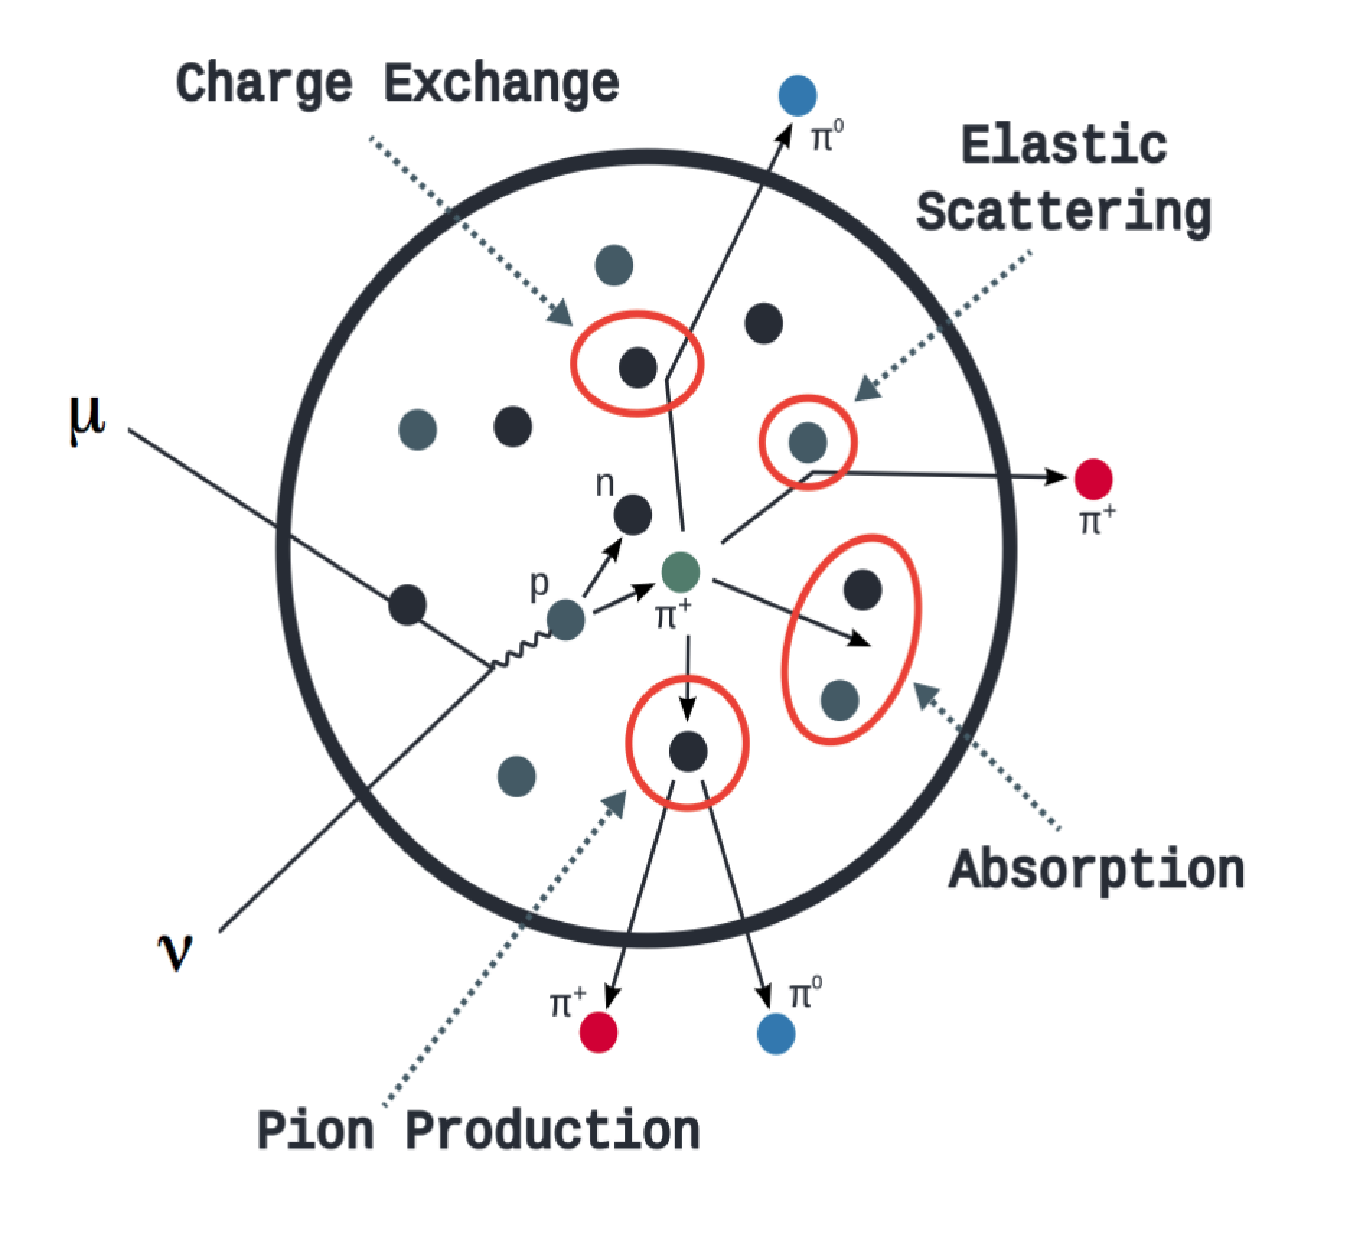
\includegraphics[width=\textwidth, trim={0mm 0mm 0mm 0mm}, clip,page=1]{Figures/Simulations/FSIDiagram.pdf}
  \end{subfigure}
  \caption{Illustration of the various processes which a pion can undergo before exiting the nucleus. Taken from \cite{10.48550/arxiv.1602.05299}.}
  \label{fig:Simulations_FSIDiagram}
\end{figure}

Any pion that is produced within the nucleus can re-interact through final state interactions before it exits, as illustrated by the scattering, absorption, production, and exchange interactions in \autoref{fig:Simulations_FSIDiagram}. These re-interactions alter the observable particles within the detector. For instance, if the charged pion from a CC PROD interaction is absorbed, the observables would mimic a CC QE interaction. To simulate these effects, NEUT uses a semi-classical intranuclear cascade model \cite{Hayato2021}. This cascade functions by stepping the pion through the nucleus in fixed-length steps equivalent to \quickmath{dx = R_{N}/100}, where \quickmath{R_{N}} is the radius of the nucleus. At each step, the simulation allows the pion to interact through scattering, charged exchange, absorption, or production with an interaction-dependent probability calculated from a fit to external data \cite{PhysRevD.99.052007}. This cascade continues until the pion is absorbed or exits the nucleus.

\subsection{Detector}

Once the final state particle kinematics have been determined by NEUT, they are passed into the detector simulation. The near detectors, ND280 and INGRID, are simulated using a \texttt{GEANT4} package \cite{t2k_det,geant4} to simulate the detector geometry, particle tracking, and energy deposition. The response of the detectors is simulated using the elecSim package \cite{t2k_det}.

The far detector simulation is based upon the original Kamiokande experiment software which uses the \texttt{GEANT3}-based SKDETSIM \cite{Brun:1987ma,t2k_det} package. This simulates the interactions of particles in the water as well as Cherenkov light production. The water quality and PMT calibration measurements detailed in \autoref{subsec:T2KSKExp_SKCalibration} are also used within this simulation to make accurate predictions of the detector response.

Any event which generates optical photons that occurs in SK will be observed by the PMT array, where each PMT records the time and accumulated charge. This recorded information is shown in event displays similar to those illustrated in \autoref{fig:Simulations_SKEventDisplays} for simulated Monte Carlo events. To be useful for physics analyses, this series of PMT hit information needs to be reconstructed to determine the number and identity of particles and their kinematics (or track parameters): four-vertex, direction, and momentum. The reconstruction uses the fact that the charge and timing distribution of photons generated by a particular particle in an event is dependent upon its initial kinematics. Electron and muon rings are distinguished by their ``fuzziness''. Muons are heavier and less affected by scattering or showering meaning they typically produce ``crisp'' rings. Electrons are more likely to interact via electromagnetic showering or scattering which results in larger variations of their direction from the initial direction. Consequently, electrons typically produce ``fuzzier'' rings compared to muons. 

\begin{figure}[h]
  \begin{subfigure}[t]{0.5\textwidth}
    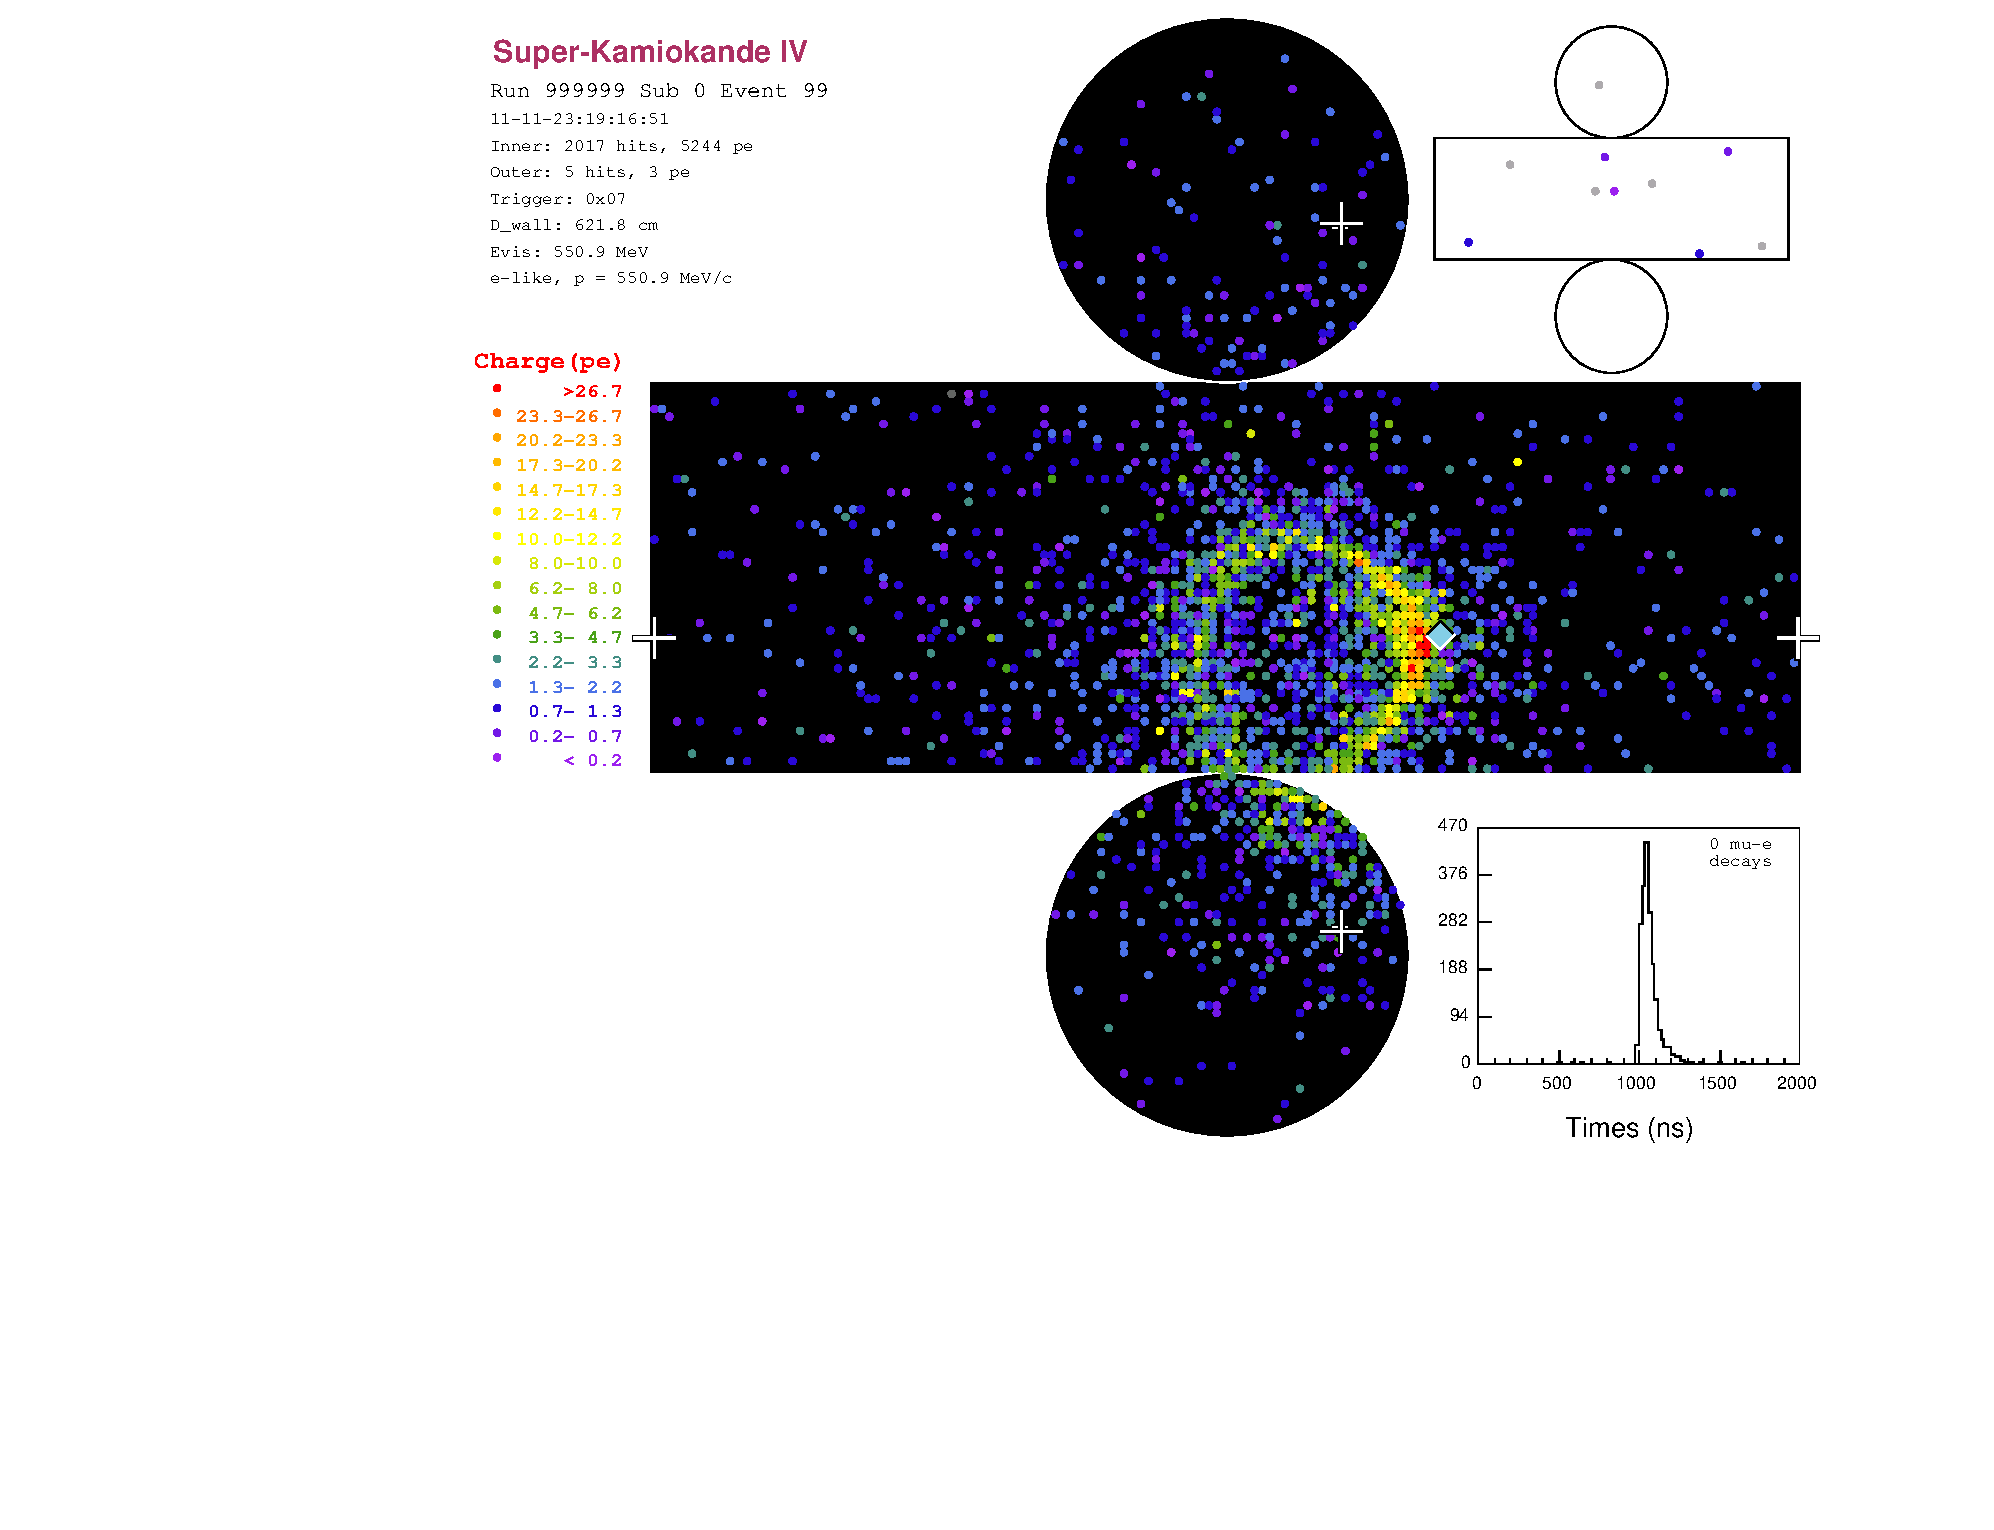
\includegraphics[width=\textwidth, trim={0mm 0mm 0mm 0mm}, clip,page=1]{Figures/Simulations/NuECandidate.pdf}
    \subcaption{\quickmath{\nu_{e}}}
  \end{subfigure}%
  \begin{subfigure}[t]{0.5\textwidth}
    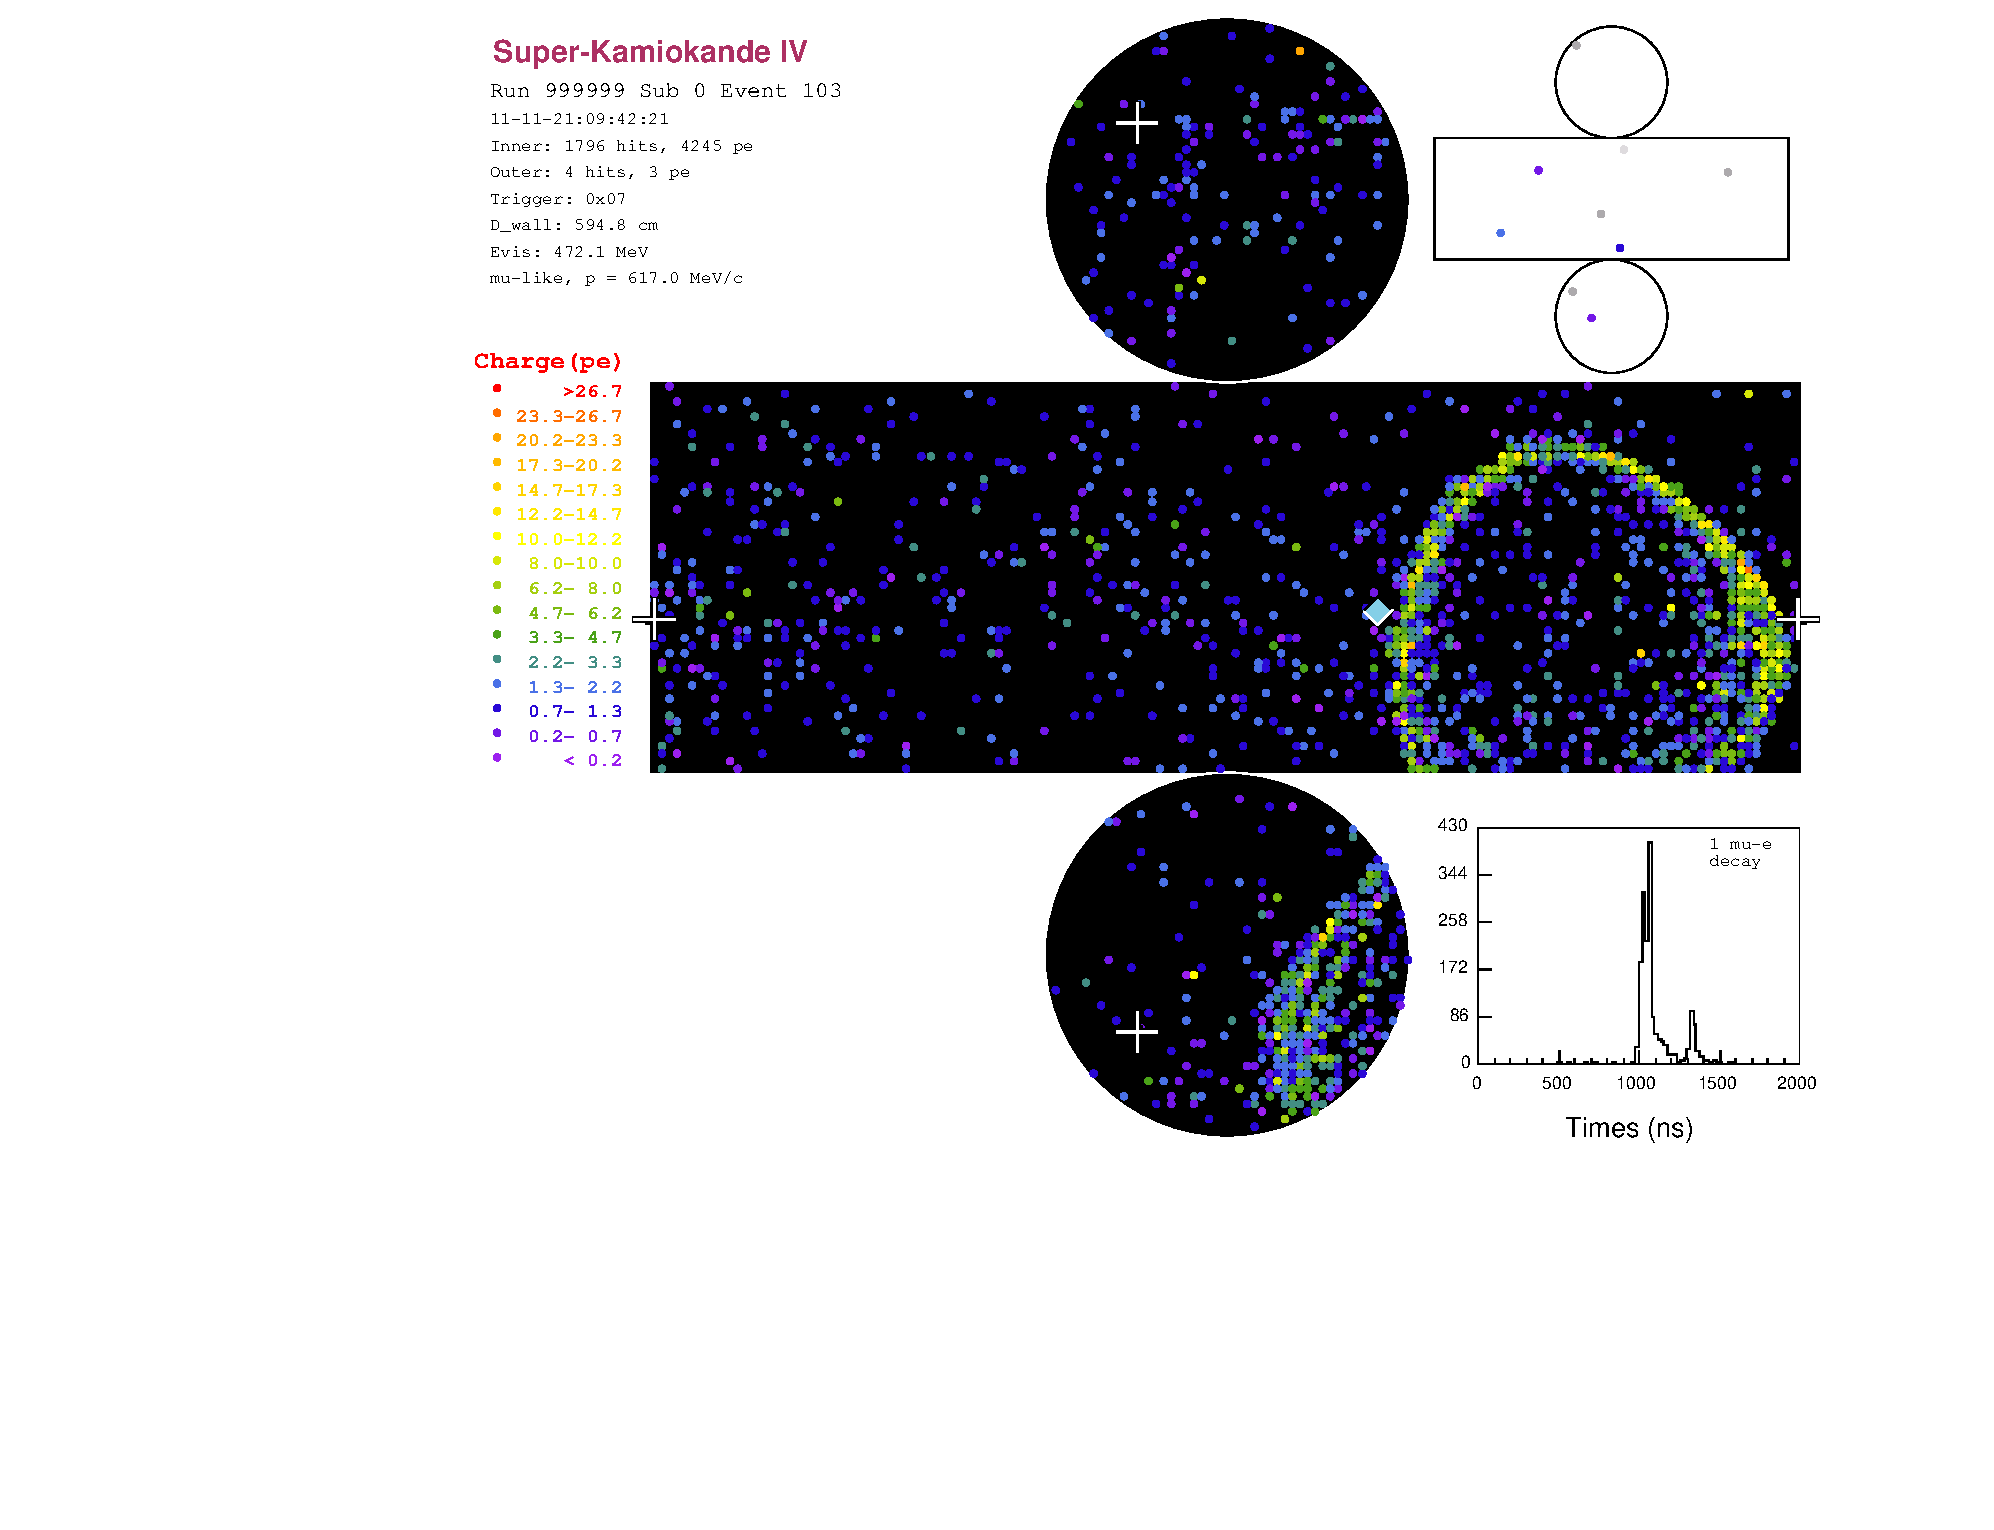
\includegraphics[width=\textwidth, trim={0mm 0mm 0mm 0mm}, clip,page=1]{Figures/Simulations/NuMuCandidate.pdf}
    \subcaption{\quickmath{\nu_{\mu}}}
  \end{subfigure}
  \caption{Event displays from Monte Carlo simulation at Super Kamiokande illustrating the ``crisp'' ring from a muon and the typically ``fuzzier'' electron ring. Each pixel represents a PMT and the color scheme denotes the accumulated charge deposited on that PMT. Figures taken from \cite{t2k_tn_219}.}
  \label{fig:Simulations_SKEventDisplays}
\end{figure}

\newpage
\section{Event Reconstruction at SK}
\label{sec:Simulation_Reconstruction}

%For the purposes of this analysis, the \texttt{fiTQun} reconstruction algorithm is utilised. Its core function is to compare a prediction of the accumulated charge and timing distribution from each PMT, generated for a particular particle identity and track parameters, to that observed in the neutrino event. It determines the preferred values by minimising a likelihood function which includes information from PMTs which were hit and those that were not hit. The \texttt{fiTQun} algorithm improves upon the \texttt{APFit} reconstruction algorithm which has been used for many previous SK analyses. \texttt{APFit} fits the vertex from timing information and then fits the momentum and direction of the particle from PMT hits within a \quickmath{43\deg} Cherenkov cone (which assumes an ultra-relativistic particle). It then fits the particle identity once the track parameters have been fit. Conversely, \texttt{fiTQun} performs a simultaneous fit of particle kinematics and identity, improving both the accuracy of the fit parameters and the rejection of neutral current \quickmath{\pi^{0}} events \cite{Abe2018, Abe2015}. The \texttt{fiTQun} algorithm is based on the key concepts of the MiniBooNE reconstruction algorithm \cite{Patterson_2009} and is described in \cite{t2k_tn_146} which is summarised below.

%An event in SK can consist of multiple ``sub-events''. For example, a muon neutrino interaction will generate a muon which will subsequently decay into an electron. Both the muon and electron can generate Cherenkov photons but both subevents need to be reconstructed separately. Therefore, to avoid assigning photons generated by the decay-electron to the muon, each event is divided into time clusters, termed ``subevents'', where subevent is defined to contain at most one hit for each PMT. To find the subevents, a vertex goodness metric is calculated for some vertex position \quickmath{\vec{x}} and time \quickmath{t},

\finish{Better separate FiTQun and APFit from the below paragraph, and add a little more information about APFit - Hough transform}

For the purposes of this analysis, the \texttt{fiTQun} reconstruction algorithm \cite{t2k_tn_146} is utilised. Its core function is to compare a prediction of the accumulated charged and timing distribution from each PMT, generated for a particular particle identity and track parameters, to that observed in the neutrino event. It determines the preferred values by maximising a likelihood function (or minimising a log-likelihood function) which includes information from PMTs which were hit and those that were not hit. The \texttt{fiTQun} algorithm is based on the key concepts of the MiniBooNE reconstruction algorithm \cite{Patterson_2009}.

The \texttt{fiTQun} algorithm improves upon the previous \texttt{APFit} algorithm \cite{Shiozawa1999} which has been used for many previous SK analyses. \texttt{APFit} fits the vertex from timing information and then fits the direction of the particle from PMT hits within a \quickmath{43\deg} Cherenkov cone (assuming an ultra-relativistic particle) using a fitting estimator. A Hough transformation is used to find the radius of a ring (related to the momentum through \autoref{eq:T2KSKExp_CherenkovConeAngle}) as well as the number of rings contained within the event. The analysis presented here uses the \texttt{fiTQun} algorithm as it improves both the accuracy of the fit parameters and the rejection of neutral current \quickmath{\pi^{0}} events as compared to \texttt{APFit} \cite{Abe2018, Abe2015}.

An event in SK can consist of prompt (or primary) and decay (or secondary) particles. For example, a charged current muon neutrino interaction can generate two particles that have the potential of generating Cherenkov photons (assuming the proton is below the Cherenkov threshold): the prompt muon, and the secondary decay-electron from the muon, approximately \quickmath{2\mu\text{s}} later. To reconstruct all particles within an event, it is divided into time clusters which are called ``subevents''. Subevents after the primary subevent are considered to be decay electrons.

The main steps of the \texttt{fiTQun} reconstruction algorithm are:

\begin{itemize}
\item \textbf{Vertex pre-fitting}: An estimate of the vertex is made using a goodness-of-fit metric based on PMT hit times
\item \textbf{Peak finding}: The initial time of each subevent is determined by clustering events by time residuals
\item \textbf{Single-ring fits}: Given the pre-fit vertex and estimated time of interaction, a maximum likelihood technique searches for a single particle generating light. Electron, muon, charged pion, and proton hypotheses are considered
\item \textbf{Multi-ring fits}: Seeded from the single-ring fits, hypotheses with multiple light-producing particles are considered using the same maximum likelihood technique. Electron-like or charged pion-like rings are added until the likelihood stops improving
\end{itemize}

To find all the subevents in an event, a vertex goodness metric is calculated for some vertex position \quickmath{\vec{x}} and time \quickmath{t},

%The number of subevents is equal to the number of decay electrons plus one (the primary event).

\begin{equation}
  G(\vec{x},t) = \sum^{\text{hit PMTs}}_{i} \exp \left( - \frac{1}{2} \left( \frac{T_{Res}^{i}(\vec{x},t)}{\sigma} \right)^{2} \right),
\end{equation}

where

\begin{equation}
  T_{Res}^{i}(\vec{x},t) = t^{i} - t - \left| R^{i}_{PMT} - \vec{x} \right|/c_{n},
\end{equation}

is the residual hit time. It is the difference in time between the PMT hit time \quickmath{t^{i}}, of the \quickmath{i^{th}} PMT, and the expected time of the PMT hit if the photon was at the vertex. \quickmath{R^{i}_{PMT}} is the position of the \quickmath{i^{th}} PMT, \quickmath{c_{n}} is the speed of light in water and \quickmath{\sigma = 4\text{ns}} which is comparable to the time resolution of the PMT. When the proposed fit values of time and vertex are close to the true values, \quickmath{T_{Res}^{i}(\vec{x},t)} tends to zero resulting in subevents appearing as spikes in the goodness metric. The proposed fit vertex and time are grid-scanned, and the values which maximise the goodness metric are selected as the ``pre-fit vertex''. Whilst this predicts a vertex for use in the clustering algorithm, the final vertex is fit using the higher-precision maximum likelihood method described below.

Once the pre-fit vertex has been determined, the goodness metric is scanned as a function of \quickmath{t} to determine the number of subevents. A peak-finding algorithm is then used on the goodness metric, requiring the goodness metric to exceed some threshold and drop below a reduced threshold before any subsequent additional peaks are considered. The thresholds are set such that the rate of false peak finding is minimised while still attaining good data to Monte Carlo agreement. To improve performance, the pre-fit vertex for each delayed subevent is re-calculated after PMT hits from the previous subevent are masked. This improves the decay-electron tagging performance. Once all subevents have been determined, the time window around each subevent is then defined by the earliest and latest time which satisfies \quickmath{-180 < T_{Res}^{i} < 800 \text{ns}}. The subevents and associated time windows are then used as seeds for further reconstruction.

For a given subevent, the \texttt{fiTQun} algorithm constructs a likelihood based on the accumulated charge \quickmath{q_{i}} and time information \quickmath{t_{i}} from the \quickmath{i^{th}} PMT,

\begin{equation}
  L(\Gamma, \vec{\theta}) = \prod^{\text{unhit}}_{j} P_{j}(\text{unhit}|\Gamma,\vec{\theta}) \prod^{\text{hit}}_{i} \{ 1 - P_{i}(\text{unhit}|\Gamma,\vec{\theta}) \}   f_{q}(q_{i} | \Gamma, \vec{\theta}) f_{t}(t_{i} | \Gamma, \vec{\theta}).
\end{equation}

Where \quickmath{\vec{\theta}} defines the track parameters; vertex position, direction vector and momenta, and \quickmath{\Gamma} represents the particle hypothesis. \quickmath{P_{i}(\text{unhit}|\Gamma,\vec{\theta})} is the probability of the \quickmath{i^{th}} tube to not register a hit given the track parameters and particle hypothesis. The charge likelihood, \quickmath{f_{q}(q_{i} | \Gamma, \vec{\theta})}, and time likelihood, \quickmath{f_{t}(t_{i} | \Gamma,\vec{\theta})}, represents the probability density function of observing charge \quickmath{q_{i}} and time \quickmath{t_{i}} on the \quickmath{i^{th}} PMT given the specified track parameters and particle hypothesis.

%As the generation and propagation of the optical photons are independent of the PMT and electronics response, it is natural to split the calculation into two. This split was also performed to . Firstly, the expected number of photoelectrons (or predicted charge), \quickmath{\mu_{i} = \mu_{i}(\vec{\theta},\Gamma)}, at the \quickmath{i^{th}} PMT is calculated. This value is then substituted into the likelihood function. This allows the charge likelihood density \quickmath{f_{q}(q_{i} | \mu_{i})} and unhit probability \quickmath{P_{i}(\text{unhit}|\mu_{i})} to be expressed via quantities that are only dependent on the response of the PMT. 

The predicted charge is calculated based on contributions from both the direct light and the scattered light. The direct light contribution is determined based on the integration of the Cherenkov photon profile along the track. PMT angular acceptance, water quality, and calibration measurements discussed in \autoref{subsec:T2KSKExp_SKCalibration} are included to accurately predict the charge probability density at each PMT. The scattered and reflected light is calculated in a similar way, although it includes a scattering function that depends on the vertex of the particle and the position of the PMT. The charge likelihood is calculated by comparing the prediction to the observed charge in the PMT which is tuned to the PMT simulation.

The time likelihood is approximated to depend on the vertex \quickmath{\vec{x}}, direction \quickmath{\vec{d}}, and time \quickmath{t} of the track as well as the particle hypothesis. The expected time for PMT hits is calculated by assuming unscattered photons being emitted from the midpoint of the track, \quickmath{S_{mid}},

\begin{equation}
  t_{exp}^{i} = t + S_{mid}/c + |R_{PMT}^{i} - \vec{x} - S_{mid}\vec{d}|/c_{n},
\end{equation}

where \quickmath{c} is the speed of light in a vacuum. The time likelihood is then expressed in terms of the residual difference between the PMT hit time and the expected hit time, \quickmath{t_{Res}^{i} = t^{i} - t_{exp}^{i}}.
%As the first photon hit defines the PMT hit time, the time likelihood density profile is narrower for higher momenta particles which introduces a dependence on the predicted charge.
The particle hypothesis and momentum also affect the Cherenkov photon distribution. These parameters modify the shape of the time likelihood density since in reality not all photons are emitted at the midpoint of the track. As with the charge likelihood, the contributions from both the direct and scattered light to the time likelihood density are calculated separately, which are both calculated from particle gun Monte Carlo studies.

The track parameters and particle identity which maximise \quickmath{L(\Gamma , \vec{\theta})} are defined as the best-fit parameters. In practice MINUIT \cite{James:2296388} is used to minimise the value of \quickmath{-\ln L(\Gamma, \vec{\theta})}. The \texttt{fiTQun} algorithm considers an electron-like, muon-like, and charged pion-like hypothesis for events with a single final state particle, denoted ``single-ring events''. The particle's identity is determined by taking the ratio of the likelihood of each of the hypotheses. For instance, electrons and muons are distinguished by considering the value of \quickmath{\ln \left( L(e,\vec{\theta}_{e})/L(\mu,\vec{\theta}_{\mu}) \right)} in comparison to the reconstructed momentum of the electron hypothesis, as illustrated by \autoref{fig:Simulations_LLHDiscriminator}. The coefficients of the discriminator between electron-like and muon-like events are determined from Monte Carlo studies \cite{t2k_tn_146}. Similar distributions exist for distinguishing electron-like events from \quickmath{\pi^{0}}-like events, and muon-like events from pion-like events. The cuts are defined as,

\begin{align}
  \begin{split}
    \text{Electron/Muon} &: \ln(L_{e}/L_{\mu}) > 0.2 \times p_{e}^{rec} [\text{MeV}], \\
    \text{Electron/\quickmath{\pi^{0}}} &: \ln(L_{e}/L_{\pi^{0}}) < 175 - 0.875 \times m_{\gamma\gamma} [\text{MeV}], \\
    \text{Muon/Pion} &: \ln(L_{\mu}/L_{\pi^{\pm}}) < 0.15 \times p_{\mu}^{rec} [\text{MeV}], \\
  \end{split}
\end{align}

as taken from \cite{t2k_tn_319}, where \quickmath{p_{e}^{rec}} and \quickmath{p_{\mu}^{rec}} are the reconstructed momentum of the single-ring electron and muon fits, respectively. \quickmath{m_{\gamma\gamma}} represents the reconstructed invariant mass of the two photons emitted from \quickmath{\pi^{0}} decay. Typically, the distance between a particular entry in these two-dimensional distributions and the cut-line is termed the PID parameter and is illustrated in \autoref{fig:Simulations_EMUPIDParamDistribution}.

\begin{figure}[h]
  \begin{subfigure}[t]{1.1\textwidth}
    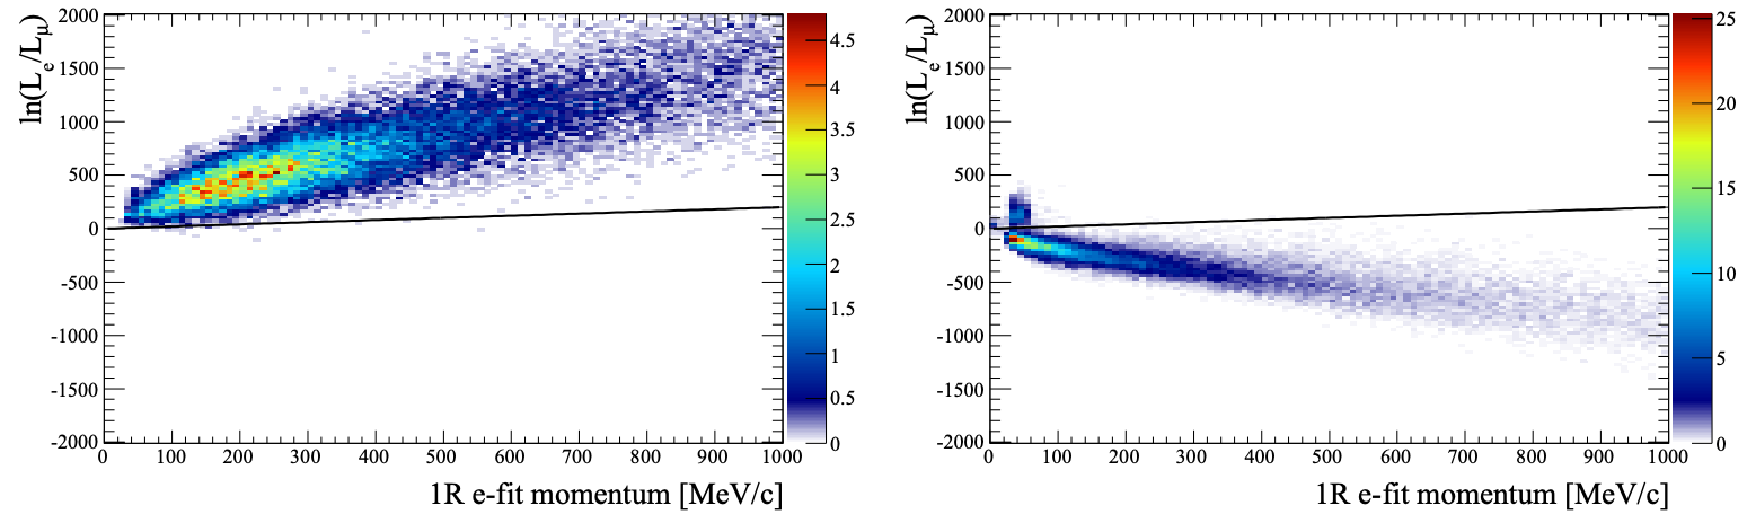
\includegraphics[width=\textwidth, trim={0mm 0mm 0mm 0mm}, clip, page=1]{Figures/Simulations/LogLikelihoodDiscriminator.pdf}
  \end{subfigure}
  \caption{The difference of the electron-like and muon-like log-likelihood compared to the reconstructed single-ring fit momentum for atmospheric \quickmath{\nu_{e}} (left) and \quickmath{\nu_{\mu}} (right) samples. The black line represents the cut used to discriminate electron-like and muon-like events, with coefficients obtained from Monte Carlo studies. Figures from \cite{t2k_tn_146}.}
  \label{fig:Simulations_LLHDiscriminator}
\end{figure}

\begin{figure}[h]
  \begin{subfigure}[t]{0.9\textwidth}
    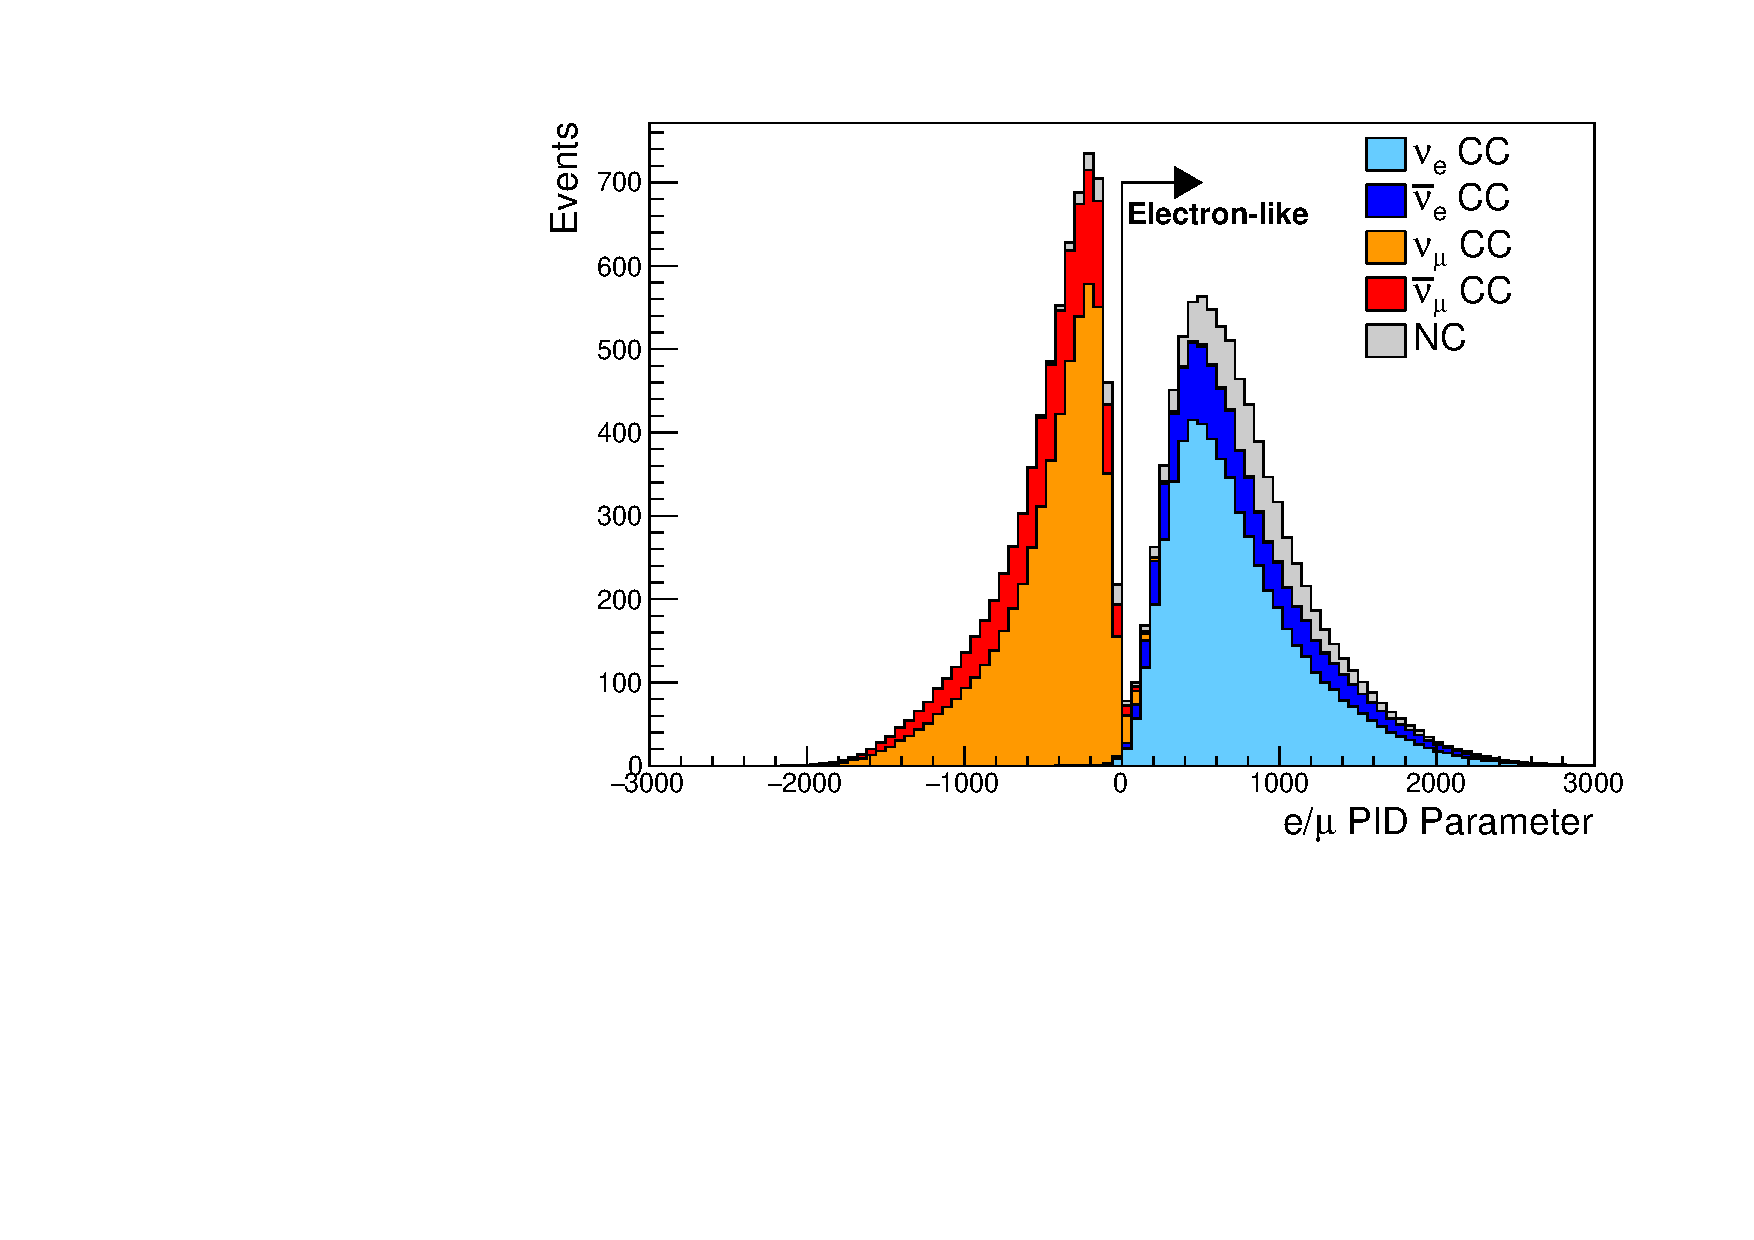
\includegraphics[width=\textwidth, trim={0mm 0mm 0mm 0mm}, clip, page=1]{Figures/Simulations/PIDParameter.pdf}
  \end{subfigure}
  \caption{The electron/muon PID separation parameter for all sub-GeV single-ring events in SK-IV. The charged current (CC) component is broken down in four flavours of neutrino (\quickmath{\nu_{\mu}}, \quickmath{\bar{\nu}_{\mu}}, \quickmath{\nu_{e}} and \quickmath{\bar{\nu}_{e}}). Events with positive values of the parameter are determined to be electron-like.}
  \label{fig:Simulations_EMUPIDParamDistribution}
\end{figure}

The \texttt{fiTQun} algorithm also considers a \quickmath{\pi^{0}} hypothesis. To do this, it performs a fit looking for two standard electron-hypothesis tracks which point to the same four-vertex. This assumes the electron tracks are generated from photon-conversion so the electron tracks actually appear offset from the proposed \quickmath{\pi^{0}} vertex. For these fits, the conversion length, direction, and momentum of each photon are also considered as track parameters which are then fit in the same methodology as the standard single-ring hypotheses. 

Whilst lower energy events are predominantly single-ring events, higher energy neutrino events can generate final states with multiple particles which generate Cherenkov photons. These ``multi-ring'' hypotheses are also considered in the \texttt{fiTQun} algorithm. When calculating the charge likelihood density, the predicted charge associated with each ring is calculated separately and then summed to calculate the total accumulated charge on each PMT. Similarly, the time likelihood for the multi-ring hypothesis is calculated assuming each ring is independent. Each track is time-ordered based on the time of flight from the center of the track to the PMT and the direct light from any ring incident on the PMT is assumed to arrive before any scattered light. To reduce computational resource usage, the multi-ring fits only consider electron-like and charged pion-like rings as the pion fit can be used as a proxy for a muon fit due to their similar mass.

\finish{Figure out how pion-like rings are different from the muon hypothesis}

Multi-ring fits proceed by proposing another ring to the previous fit and then fitting the parameters in the method described above. Typically, multi-ring fits have the largest likelihood because of the additional degrees of freedom introduced. A likelihood value is calculated for the \quickmath{n}-ring and \quickmath{(n+1)}-ring hypotheses, where the additional ring is only included if the likelihood value is above \quickmath{9.35}, based on Monte Carlo studies in \cite{Tobayama:2016dsi}.

\subsection{Validation of Reconstruction in SK-V}
\label{sec:Simulation_ReconstructionInSKV}

Understanding how the modelling of the detector conditions and stability effects the reconstruction is critical for ensuring accurate measurements. It is important to note that the detector systematics used in the 2020 T2K-only \cite{Dunne2020-uf} oscillation analysis are determined using data-to-Monte Carlo comparisons of the SK-IV data \cite{t2k_tn_399}. Due to tank-open maintenance occurring between SK-IV and SK-V, the dark rate of each PMT was observed to increase in SK-V due to light exposure for a significant time during the repairs. This increase can be seen in \autoref{fig:Simulations_DarkRateVariation}. Run-10 of the T2K experiment was conducted in the SK-V period, so the consistency of SK-IV and SK-V data needs to be studied to determine whether the SK-IV-defined systematics can be applied to the run-10 data. Consequently, the author of this thesis assessed the quality of \texttt{fiTQun} event reconstruction for SK-V data.

This comparison study was performed using the stopping muon data set for both the SK-IV and SK-V periods. This data sample is used due to the high rate of interactions (\quickmath{O(200)} events per hour) as well as having similar energies to muons from CCQE \quickmath{\nu_{\mu}} interactions from beam interactions. The rate of cosmic muons does depend on the solar activity cycle \cite{Maghrabi2021} but has been neglected in this comparison study. This is because the shape of the distributions is most important for the purposes of being compared to the detector systematics. The SK-IV and SK-V data samples consist of \quickmath{2398.42} and \quickmath{626.719} hours of data which equates to \quickmath{686\text{k}} and \quickmath{192\text{k}} events respectively. These samples do not correspond to the full data sets of either period but do contain enough events to be systematics limited rather than statistics limited.

\begin{figure}[h]
  \begin{subfigure}[t]{\textwidth}
    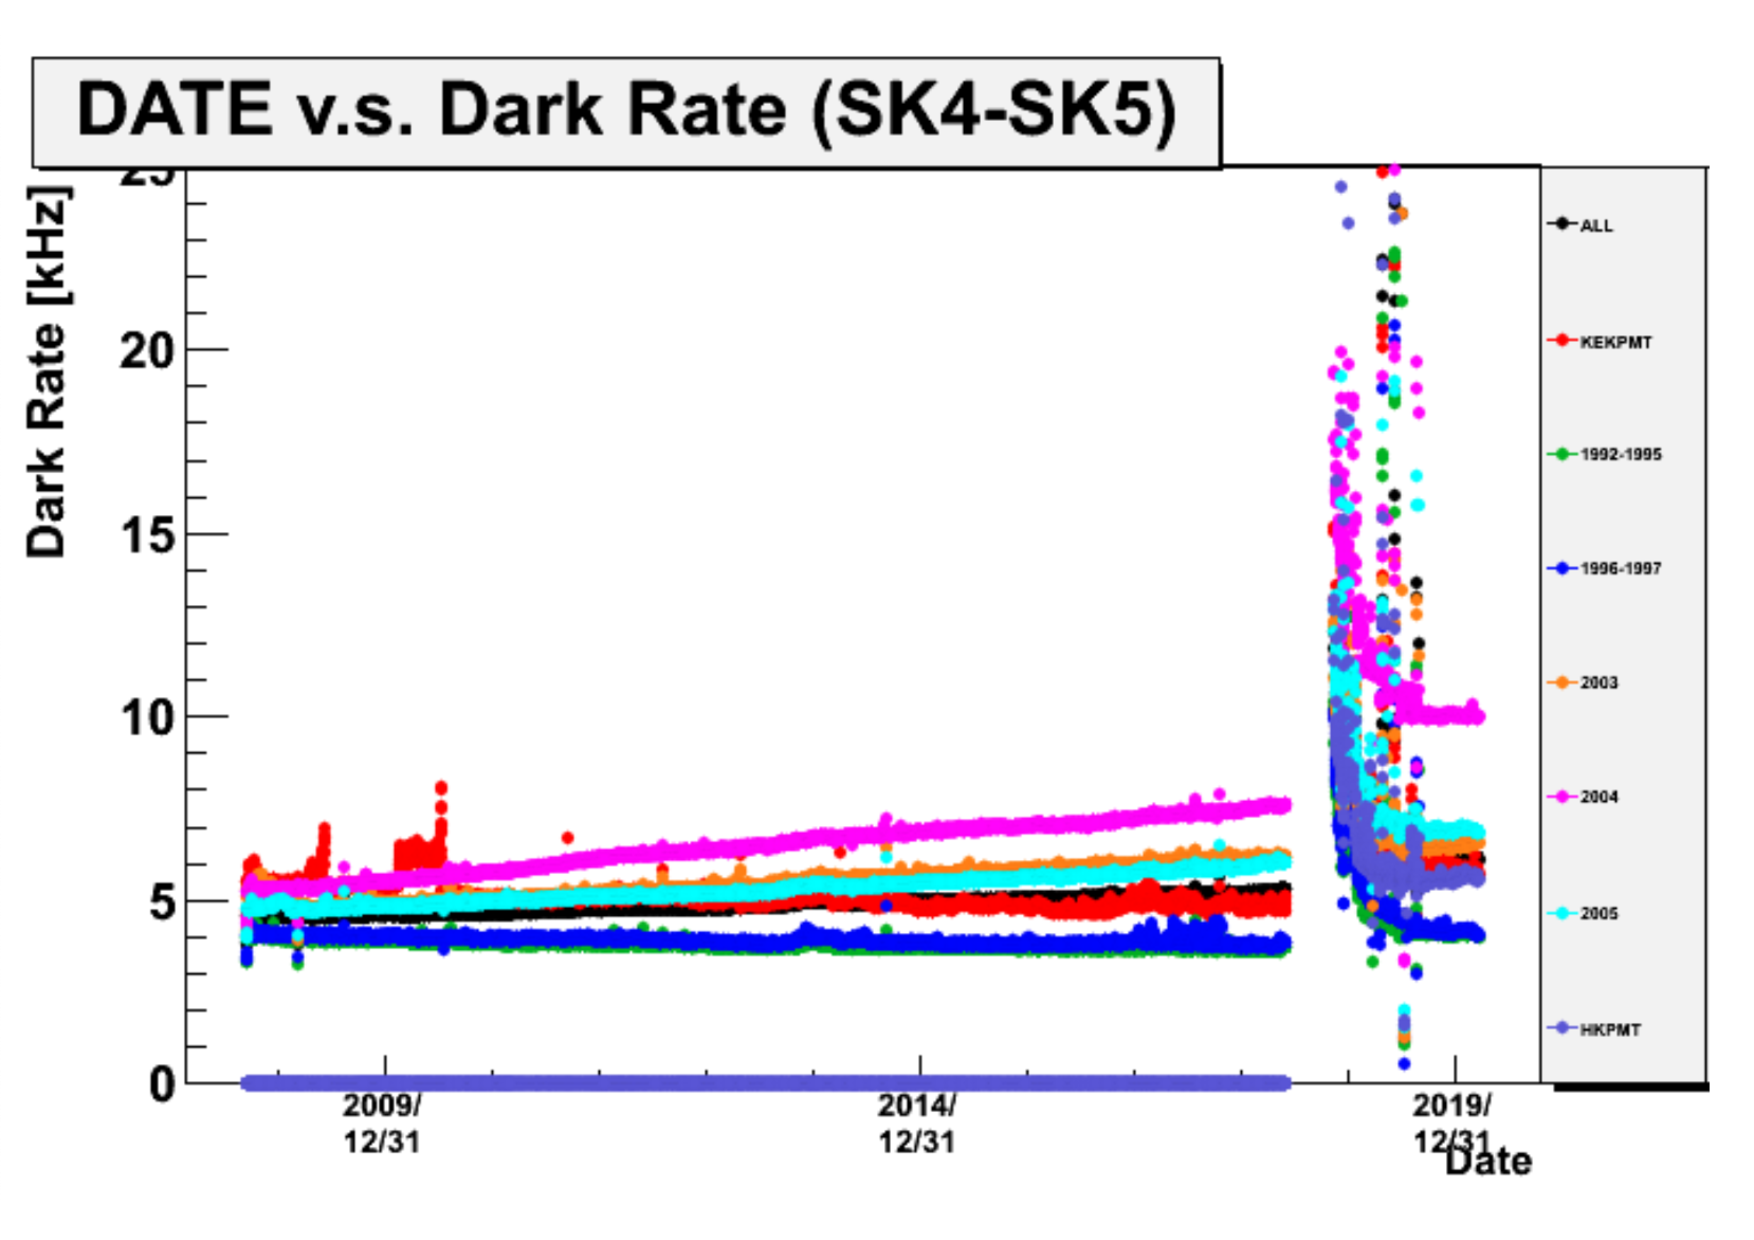
\includegraphics[width=\textwidth, trim={0mm 0mm 0mm 0mm}, clip, page=1]{Figures/Simulations/DarkRate.pdf}
  \end{subfigure}
  \caption{The variation of the measured dark rate as a function of date, broken down by PMT type. The SK-IV and SK-V periods span September 2008 to May 2018 and January 2019 to July 2020, respectively. The break in measurement in 2018 corresponds to the period of tank repair and refurbishment. Figure adapted from \cite{t2k_tn_399}.}
  \label{fig:Simulations_DarkRateVariation}
\end{figure}

The predicted charge calculated in the \texttt{fiTQun} algorithm includes a contribution from the photoelectron emission due to dark noise. Therefore, the increase in the SK-V dark rate needs to be accounted for. In practice, the average dark rate in each SK period is calculated and used as an input in the reconstruction. This is calculated by averaging the dark rate per run for each period separately, using the calibration measurements detailed in \autoref{subsec:T2KSKExp_SKCalibration}. The average dark rate from SK-IV and SK-V were found to be \quickmath{4.57\text{kHz}} and \quickmath{6.30\text{kHz}}, respectively. The charges associated with the muon and decay electron subevents are illustrated in \autoref{fig:Simulations_MeasuredChargeDistribution}. The photoelectron emission from dark noise is more significant for events that have lower energy. This is because this contribution becomes more comparable to the number of photoelectrons emitted from incident photons in lower-energy events. This behaviour is observed in the data, where the charge deposited by the muon subevent is mostly unaffected by the increase in dark rate, whilst the charge associated with the decay-electron is clearly affected.

\begin{figure}[h]
  \begin{subfigure}[t]{0.48\textwidth}
    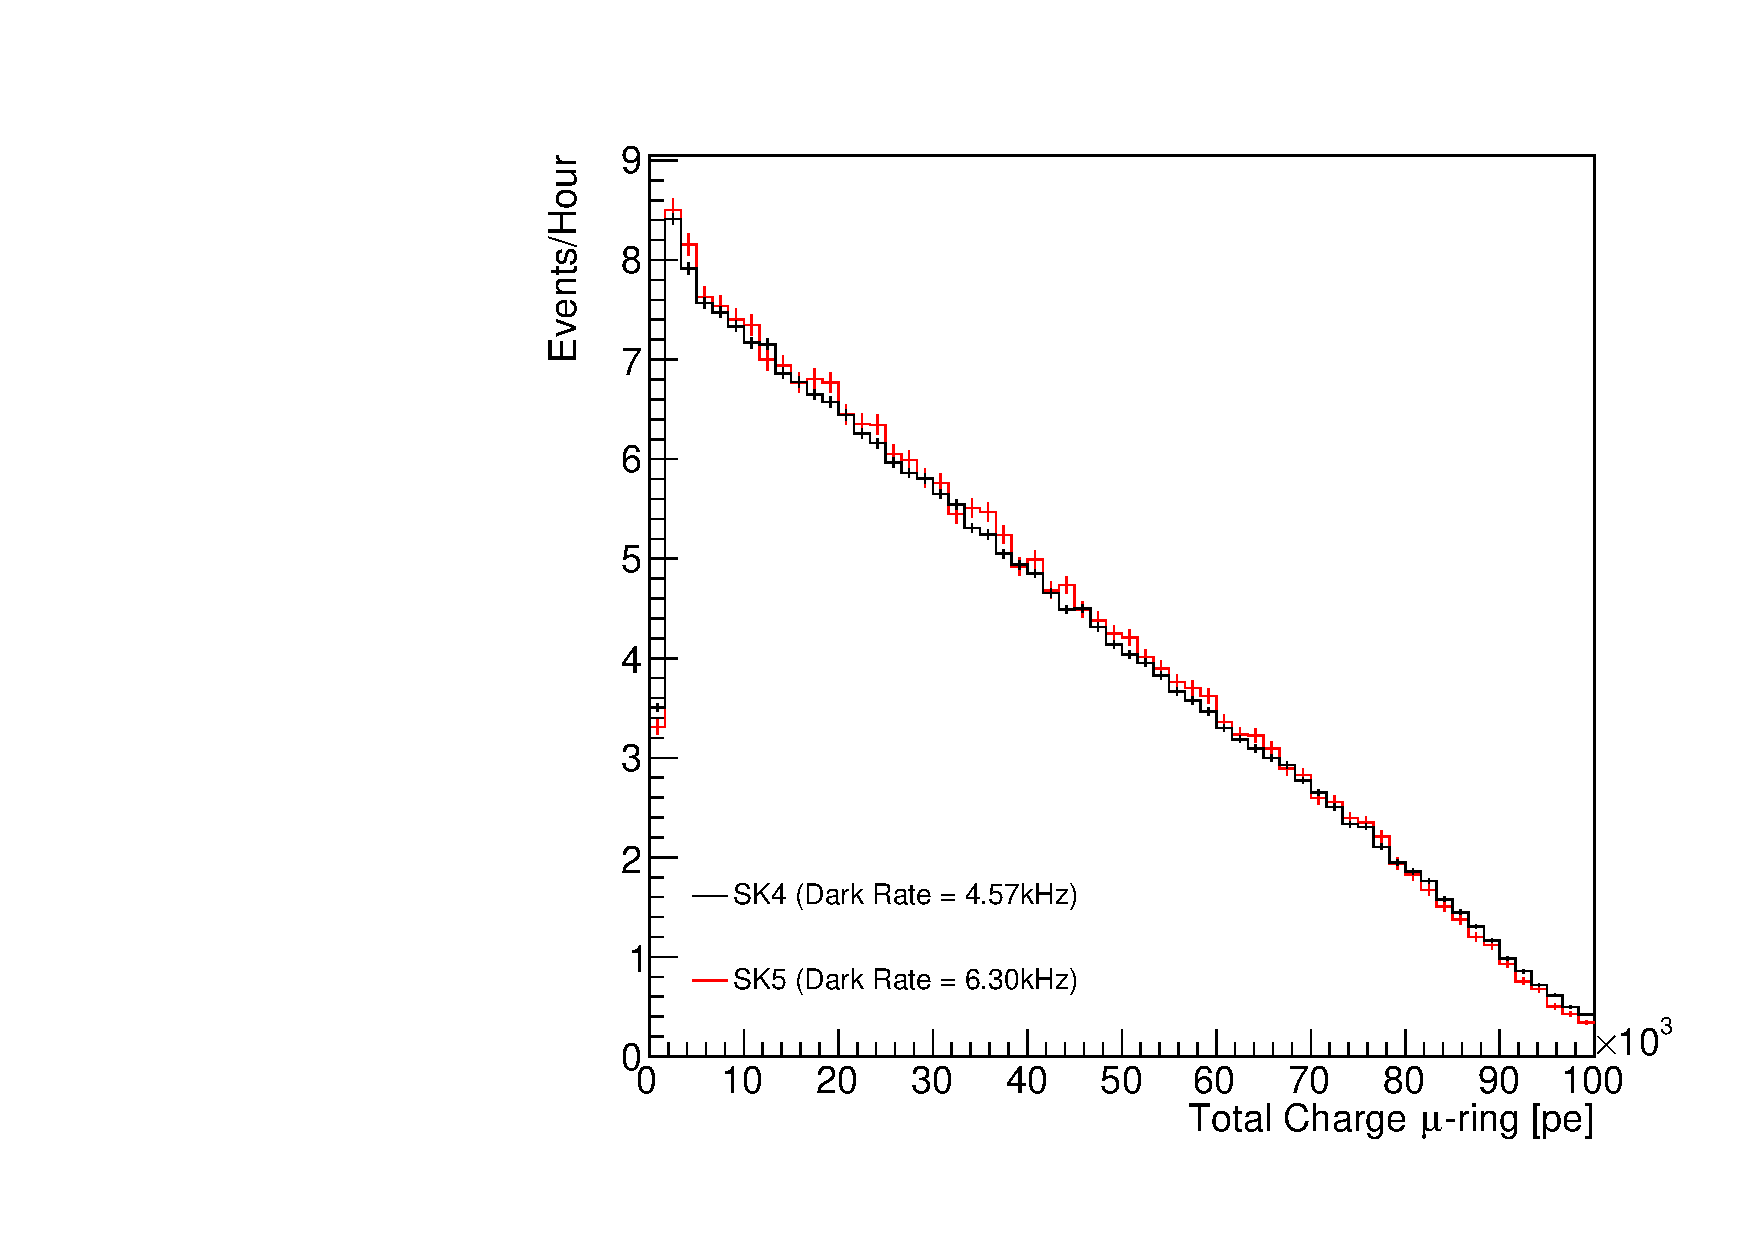
\includegraphics[width=\textwidth, trim={0mm 0mm 0mm 0mm}, clip, page=1]{Figures/Simulations/ChargeAssociatedWithMuon.pdf}
    \subcaption{Muon}
  \end{subfigure}%
  \begin{subfigure}[t]{0.48\textwidth}
    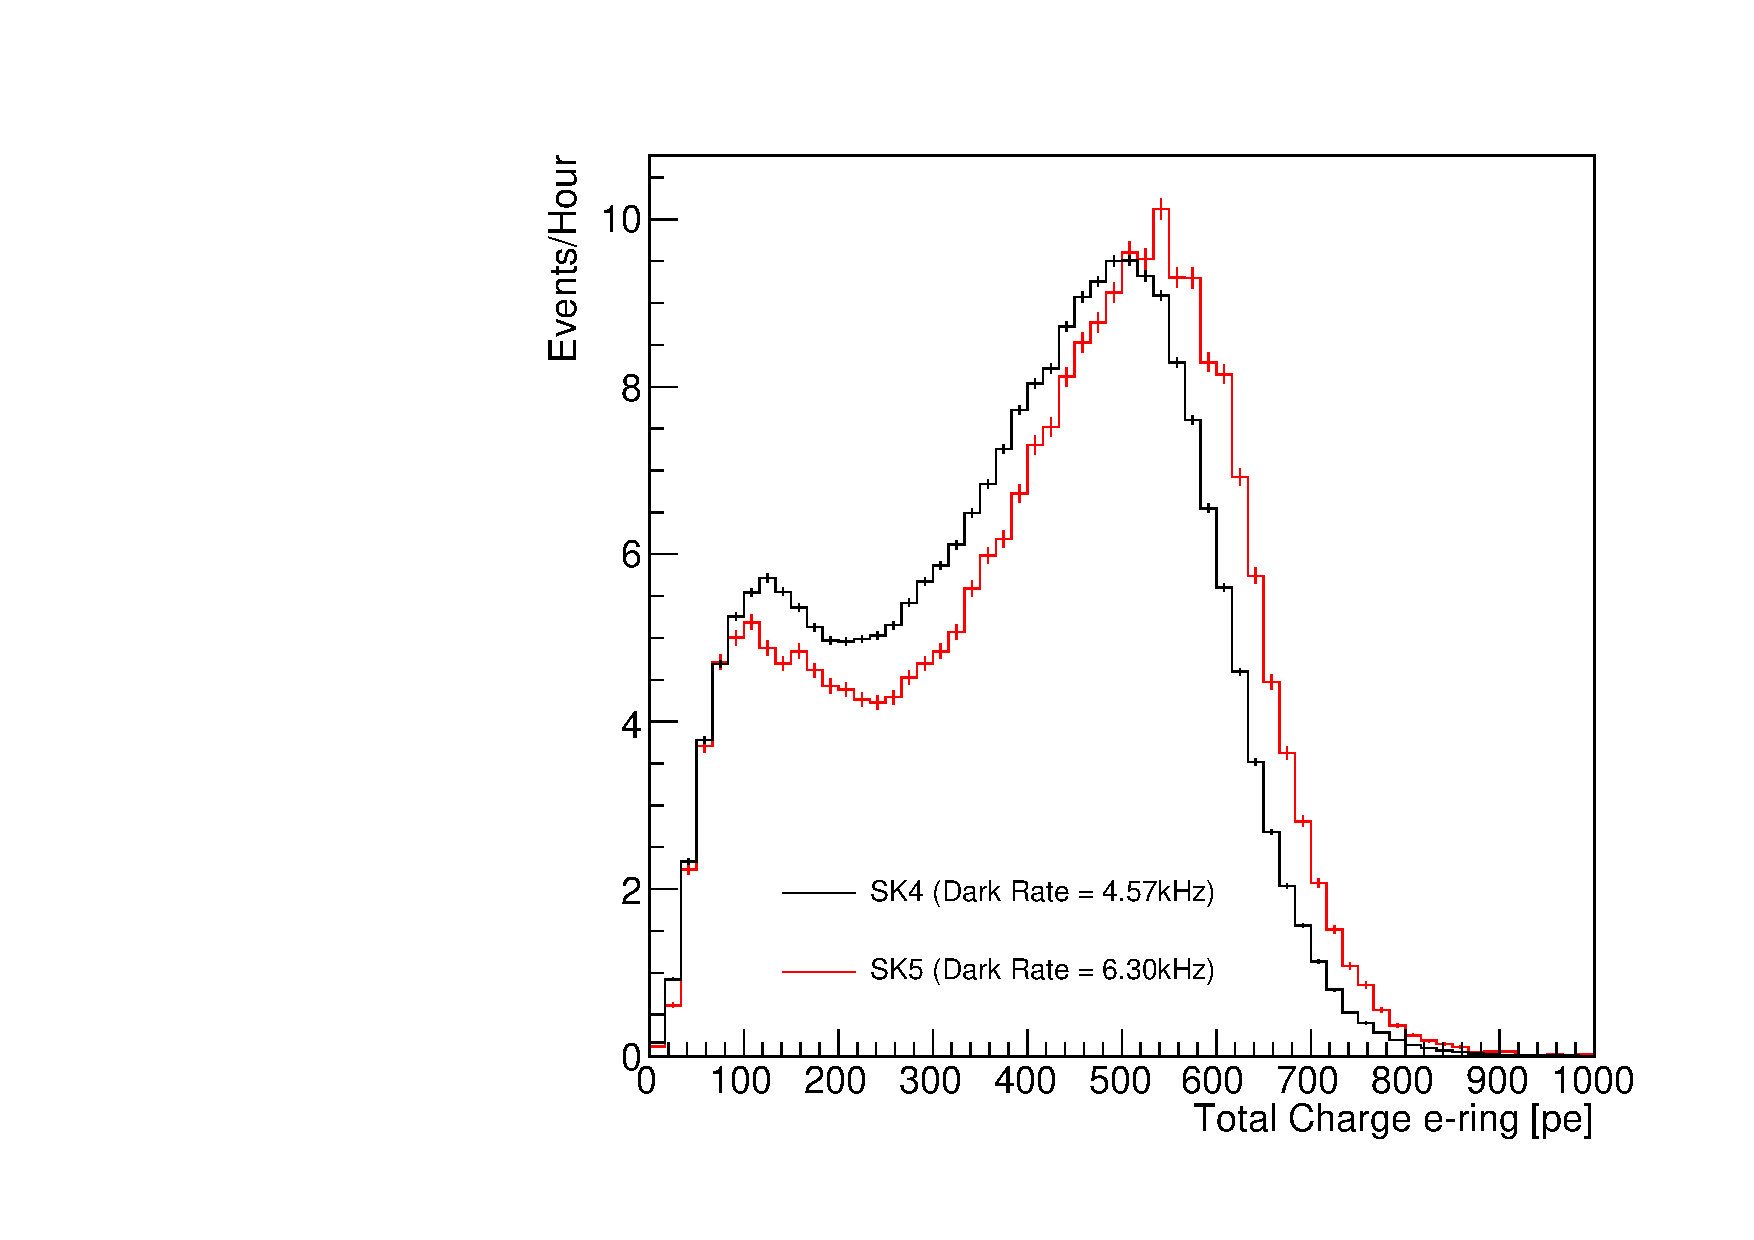
\includegraphics[width=\textwidth, trim={0mm 0mm 0mm 0mm}, clip, page=1]{Figures/Simulations/ChargeAssociatedWithDecayE.pdf}
    \subcaption{Decay Electron}
  \end{subfigure}  
  \caption{Comparison of the measured raw charge deposited per event from the stopping muon data samples between SK-IV (Blue) and SK-V (Red), split by the primary muon subevent (left) and the associated decay electron subevent (right).}
  \label{fig:Simulations_MeasuredChargeDistribution}
\end{figure}

The energy scale systematic is estimated from data-to-Monte Carlo differences in the stopping muon sample in \cite{sk_2017} and found to be \quickmath{2.1\%}. To determine the consistency of SK-IV and SK-V with respect to the energy scale systematic, the muon momentum distribution is compared between the two SK periods. As the total number of Cherenkov photons is integrated across the track length, the reconstructed momentum divided by track length (or range) is compared between SK-IV and SK-V as illustrated in \autoref{fig:Simulations_MuonMomentumByRange}.

\begin{figure}[h]
  \begin{subfigure}[t]{\textwidth}
    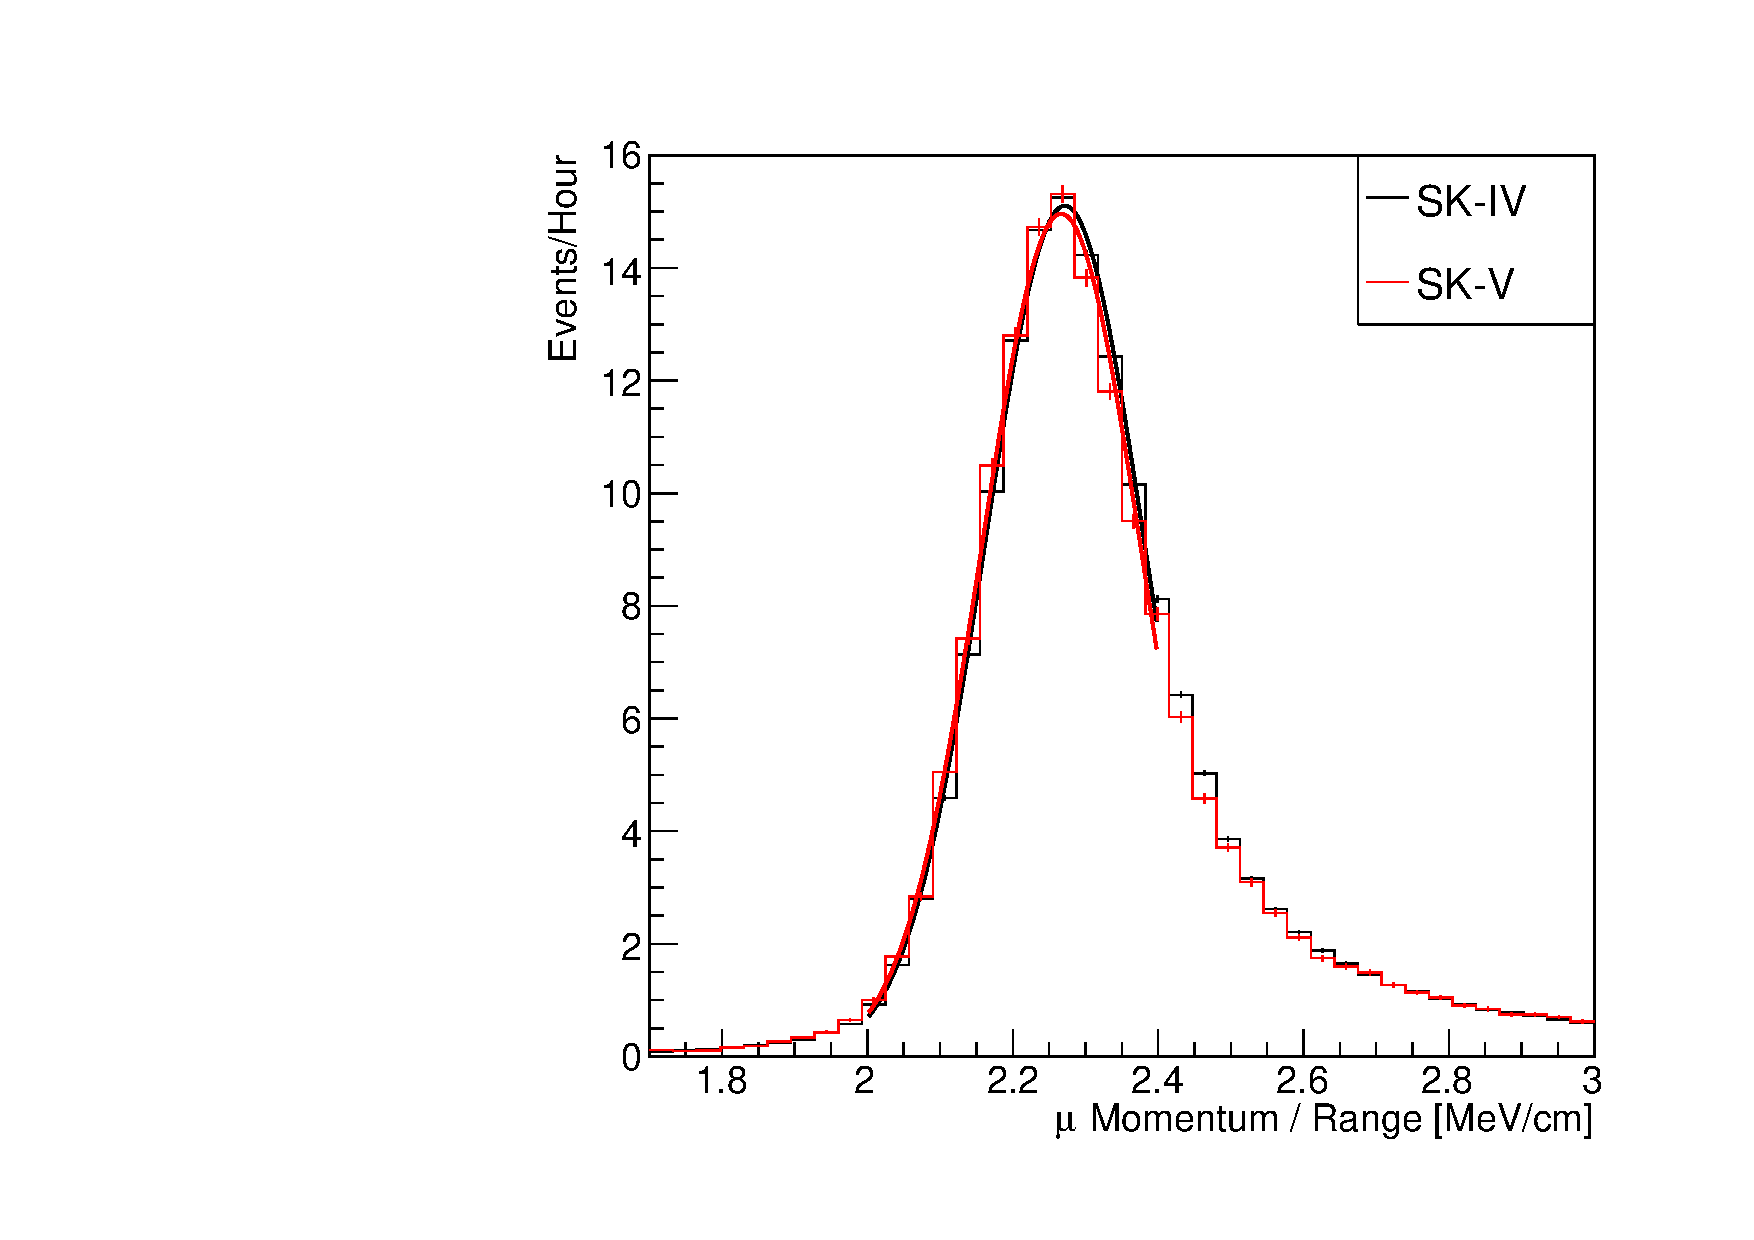
\includegraphics[width=\textwidth, trim={0mm 0mm 0mm 0mm}, clip, page=1]{Figures/Simulations/MuonRangeComparison.pdf}
  \end{subfigure}
  \caption{The distribution of the reconstructed momentum from the muon ring divided by the distance between the reconstructed muon and decay electron vertices as found in the stopping muon data sets of SK-IV (Black) and SK-IV (Red). Only events with one tagged decay electron are considered. A Gaussian fit is considered in the range \quickmath{[2.0,2.4] \text{MeV/cm}} and illustrated as the solid curve.}
  \label{fig:Simulations_MuonMomentumByRange}
\end{figure}

The consistency between these muon distributions has been computed in two ways. Firstly, a Gaussian is fit to the peak of each distribution separately, whose mean is found to be \quickmath{(2.272 \pm 0.003) \text{MeV/cm}} and \quickmath{(2.267 \pm 0.006) \text{MeV/cm}} for SK-IV and SK-V respectively. The ratio of these is equal to \quickmath{1.002 \pm 0.003}. The means of the Gaussian fits are consistent with the expected stopping power of a minimum ionising muon for a target material (water) with \quickmath{Z/A \sim 0.5} \cite{PhysRevD.86.010001}. The second consistency check is performed by introducing a nuisance parameter, \quickmath{\alpha}, which modifies the SK-V distribution. The value of \quickmath{\alpha} which minimises the \quickmath{\chi^{2}} value between the SK-IV and SK-V is determined by scanning across a range of values. This is repeated by applying the nuisance parameter as both a multiplicative factor and an additive shift. The \quickmath{\chi^{2}} distributions for different values of \quickmath{\alpha} is illustrated in \autoref{fig:Simulations_MuonMomentumByRangeChi2Scan}. The values which minimise the \quickmath{\chi^{2}} are found to be \quickmath{0.0052} and \quickmath{1.0024} for the additive and multiplicative implementations, respectively. No evidence of shifts larger than the \quickmath{2.1\%} uncertainty on the energy scale systematic has been found in the reconstructed momentum distribution of SK-IV and SK-V.

\begin{figure}[h]
  \begin{subfigure}[t]{\textwidth}
    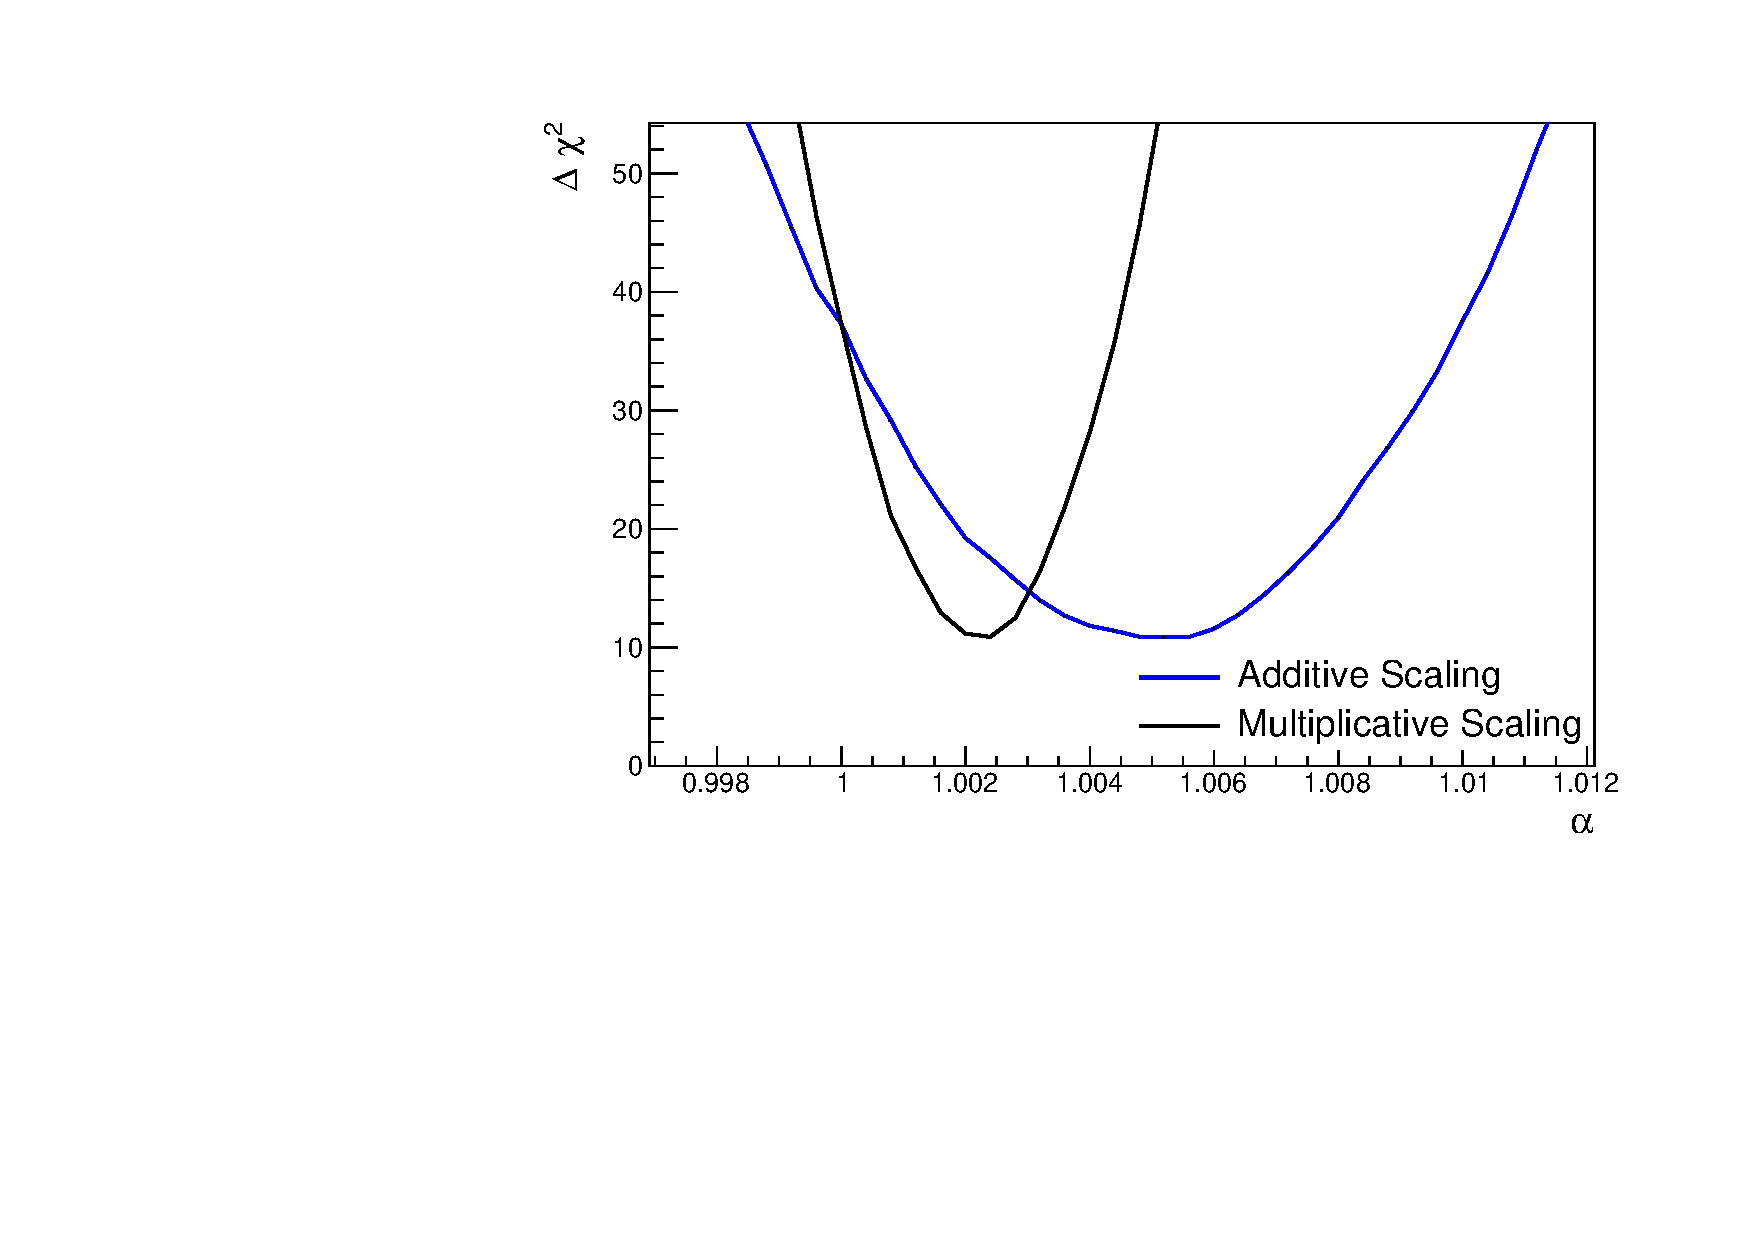
\includegraphics[width=\textwidth, trim={0mm 0mm 0mm 0mm}, clip, page=1]{Figures/Simulations/MuonRange_Chi2Scan.pdf}
  \end{subfigure}
  \caption{The \quickmath{\chi^{2}} difference between the SK-IV and SK-V reconstructed muon momentum divided by range when the SK-V is modified by the scaling parameter \quickmath{\alpha}. Both additive (Blue) and multiplicative (Black) scaling factors have been considered. In practice, the additive scaling factor actually uses the value of (\quickmath{\alpha-1.0}) but is illustrated like this so the results can be shown on the same axis range.}
  \label{fig:Simulations_MuonMomentumByRangeChi2Scan}
\end{figure}

\section{Event Reduction at SK}
\label{sec:Simulations_Reduction}

In normal data-taking operations, the SK detector observes many background events alongside the beam and atmospheric neutrino signal events of physics interest for this thesis. Cosmic ray muons and flasher events, which are the spontaneous discharge of a given PMT, contribute the largest amount of background events in the energy range relevant to this thesis.
%Lower energy analyses like DSNB searches are also subject to radioactive backgrounds \cite{Nakano_2017}.
Therefore the data recorded is reduced with the aim of removing these background events. The reduction process is detailed in \cite{Ashie_2005, Jiang2019-iw} and briefly summarised below.

Atmospheric neutrino events observed in the SK detector are categorised into three different types of samples: fully contained (FC), partially contained (PC) and up-going muon (Up-$\mu$), using PMT hit signatures in the inner and outer detector (ID and OD, respectively). To identify FC neutrino events, it is required that the neutrino interacts inside the fiducial volume of the ID and that no significant OD activity is observed. For this analysis, an event is defined to be in the fiducial volume provided the event vertex is at least $0.5$m away from the ID walls. PC events have the same ID requirements but can have a larger signal present inside the OD. Typically, only high energy muons from \quickmath{\nu_{\mu}} interactions can penetrate the ID wall. The Up-$\mu$ sample contains events where muons are created from neutrino interactions in the OD water or rock below the tank. They then propagate upwards through the detector. Downward-going muons generated from neutrino interactions above the tank are neglected because of the difficulty in separating their signature from the cosmic muon shower background. The sample categories are visually depicted in Figure \ref{fig:Simulations_AtmosphericSampleTopology}.

\begin{figure}[ht!]
    \centering
    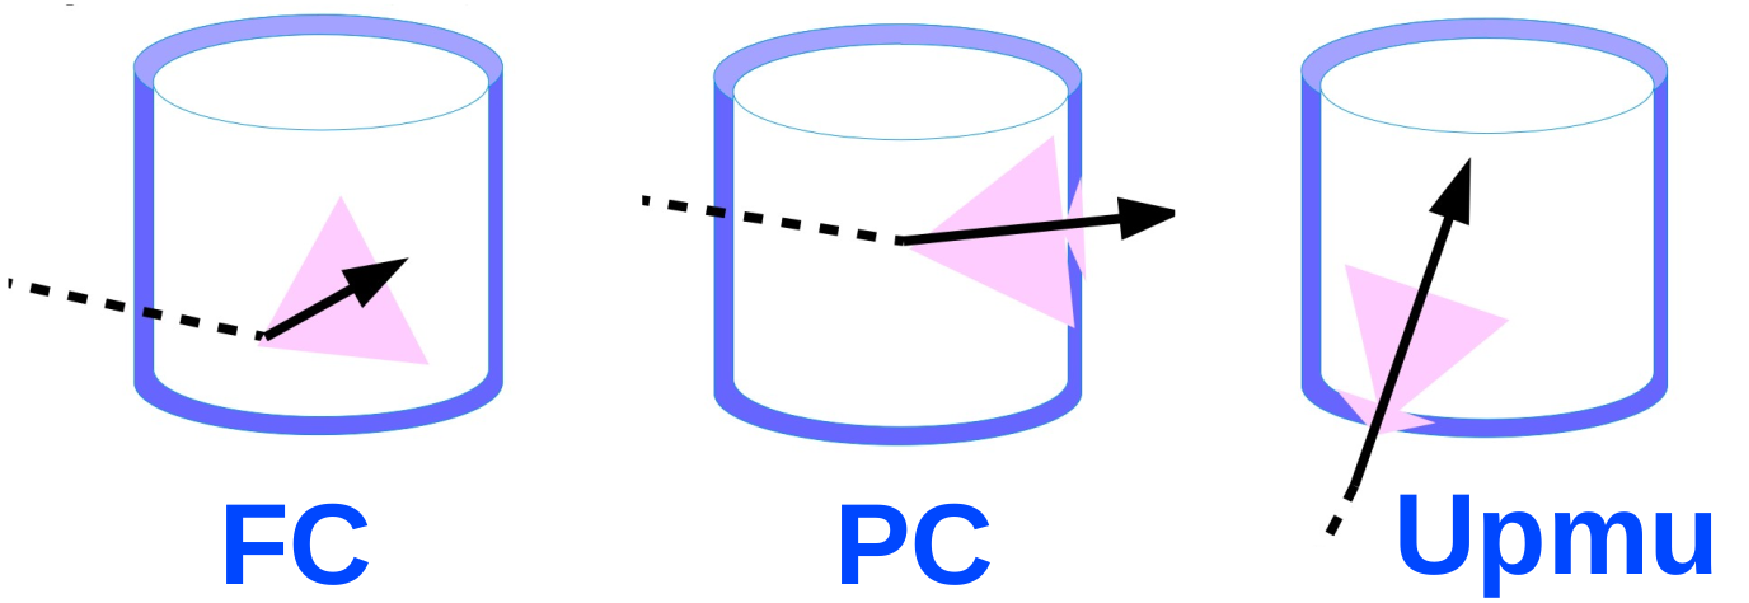
\includegraphics[width=0.8\textwidth]{Figures/Simulations/Atmo_topology.pdf}
    \caption{A depiction of the topology patterns for fully-contained (FC), partially-contained (PC), and up-going muon (\quickmath{\text{Up-}\mu}) samples included in this analysis.}
    \label{fig:Simulations_AtmosphericSampleTopology}
\end{figure}

Based on the event characteristics, as defined by the \texttt{fiTQun} event reconstruction software, the FC events are categorised by

\begin{itemize}
    \item \textbf{Visible Energy}: equal to the sum of the reconstructed kinetic energy of particles above the Cerenkov threshold for all rings present in the event. The purpose is to separate events into sub-GeV and multi-GeV categories. 
    \item \textbf{Number of observed Cerenkov rings}. The purpose is to separate single-ring and multi-ring events, where single-ring events predominantly consist of quasi-elastic interactions and multi-ring events are typically resonant pion production or deep inelastic scattering events.
    \item \textbf{Particle identification parameter of the most energetic ring}: A value determined from the maximum likelihood value based on \texttt{fiTQun}'s electron, muon, or pion hypothesis. The purpose is to separate electron-like and muon-like events.
    \item \textbf{Number of decay electrons}: The purpose is to separate quasi-elastic events (which have one decay electron emitted from the muon decay) and resonant pion production events (which have two decay electrons emitted from the muon and pion).
\end{itemize}

The PC and \quickmath{\text{Up-}\mu} categories are broken down into ``through-going'' and ``stopping'' samples depending on whether the muon leaves the detector. This is because the PC stopping events deposit the entire energy of the interaction into the detector, resulting in better reconstruction. The energy of events that exit the detector has to be estimated, with a typically worse resolution, which introduces much larger systematic uncertainties. Through-going \quickmath{\text{Up-}\mu} samples are further broken down by whether any hadronic showering was observed in the event which typically indicates DIS interactions. The expected neutrino energy for the different categories is given in \autoref{fig:Simulations_NeutrinoEnergyDistribution}. FC sub-GeV and multi-GeV events peak around \quickmath{0.7\text{GeV}} and \quickmath{3\text{GeV}} respectively, with slightly different peak energies for \quickmath{\nu_{e}} and \quickmath{\nu_{\mu}} oscillation channels. PC and \quickmath{\text{Up-}\mu} are almost entirely comprised of \quickmath{\nu_{\mu}} events and peak around \quickmath{7\text{GeV}} and \quickmath{100\text{GeV}}, respectively.

\begin{figure}[h]
  \begin{subfigure}[t]{0.49\textwidth}
    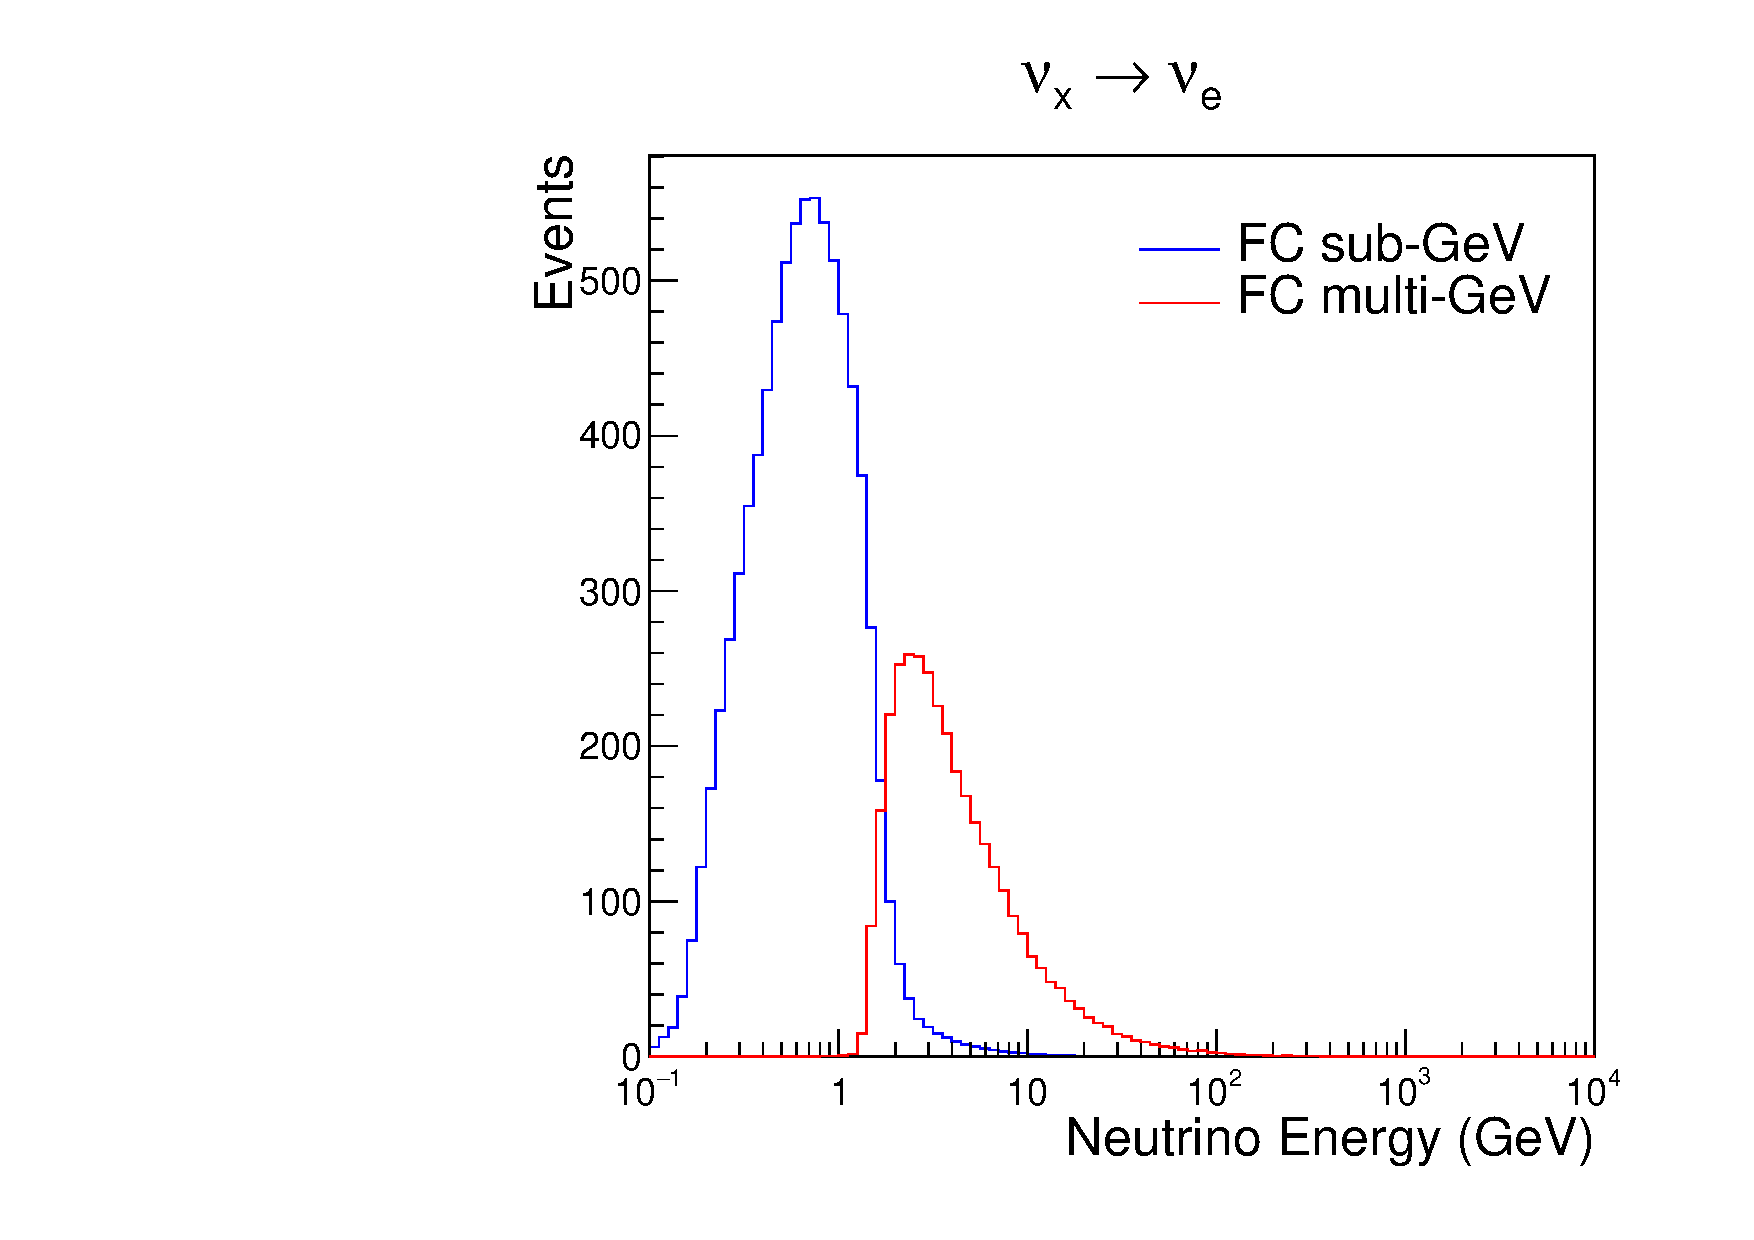
\includegraphics[width=\textwidth, trim={0mm 0mm 0mm 0mm}, clip,page=1]{Figures/Simulations/NeutrinoEnergyDist_NuE.pdf}
  \end{subfigure}%
  \begin{subfigure}[t]{0.49\textwidth}
    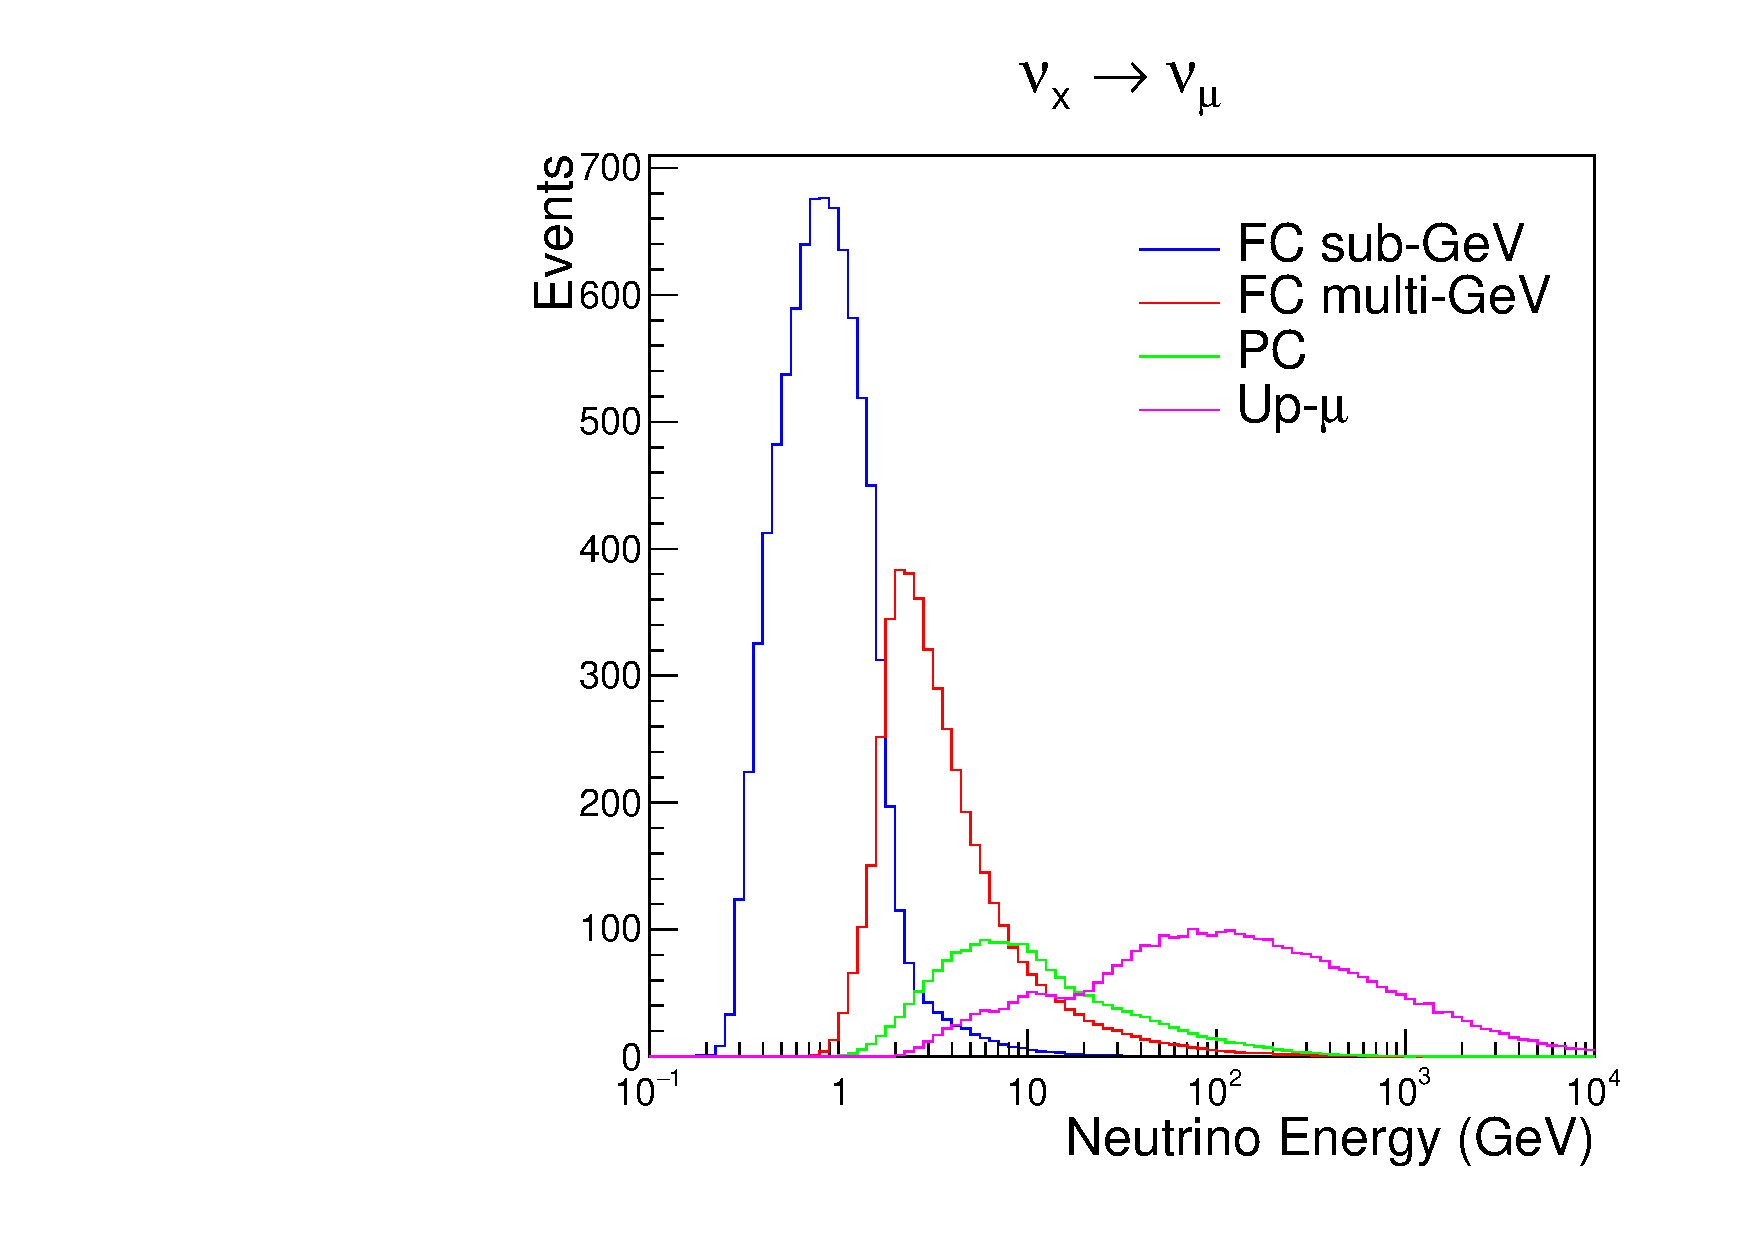
\includegraphics[width=\textwidth, trim={0mm 0mm 0mm 0mm}, clip,page=1]{Figures/Simulations/NeutrinoEnergyDist_NuMu.pdf}
  \end{subfigure}
  \begin{subfigure}[t]{0.49\textwidth}
    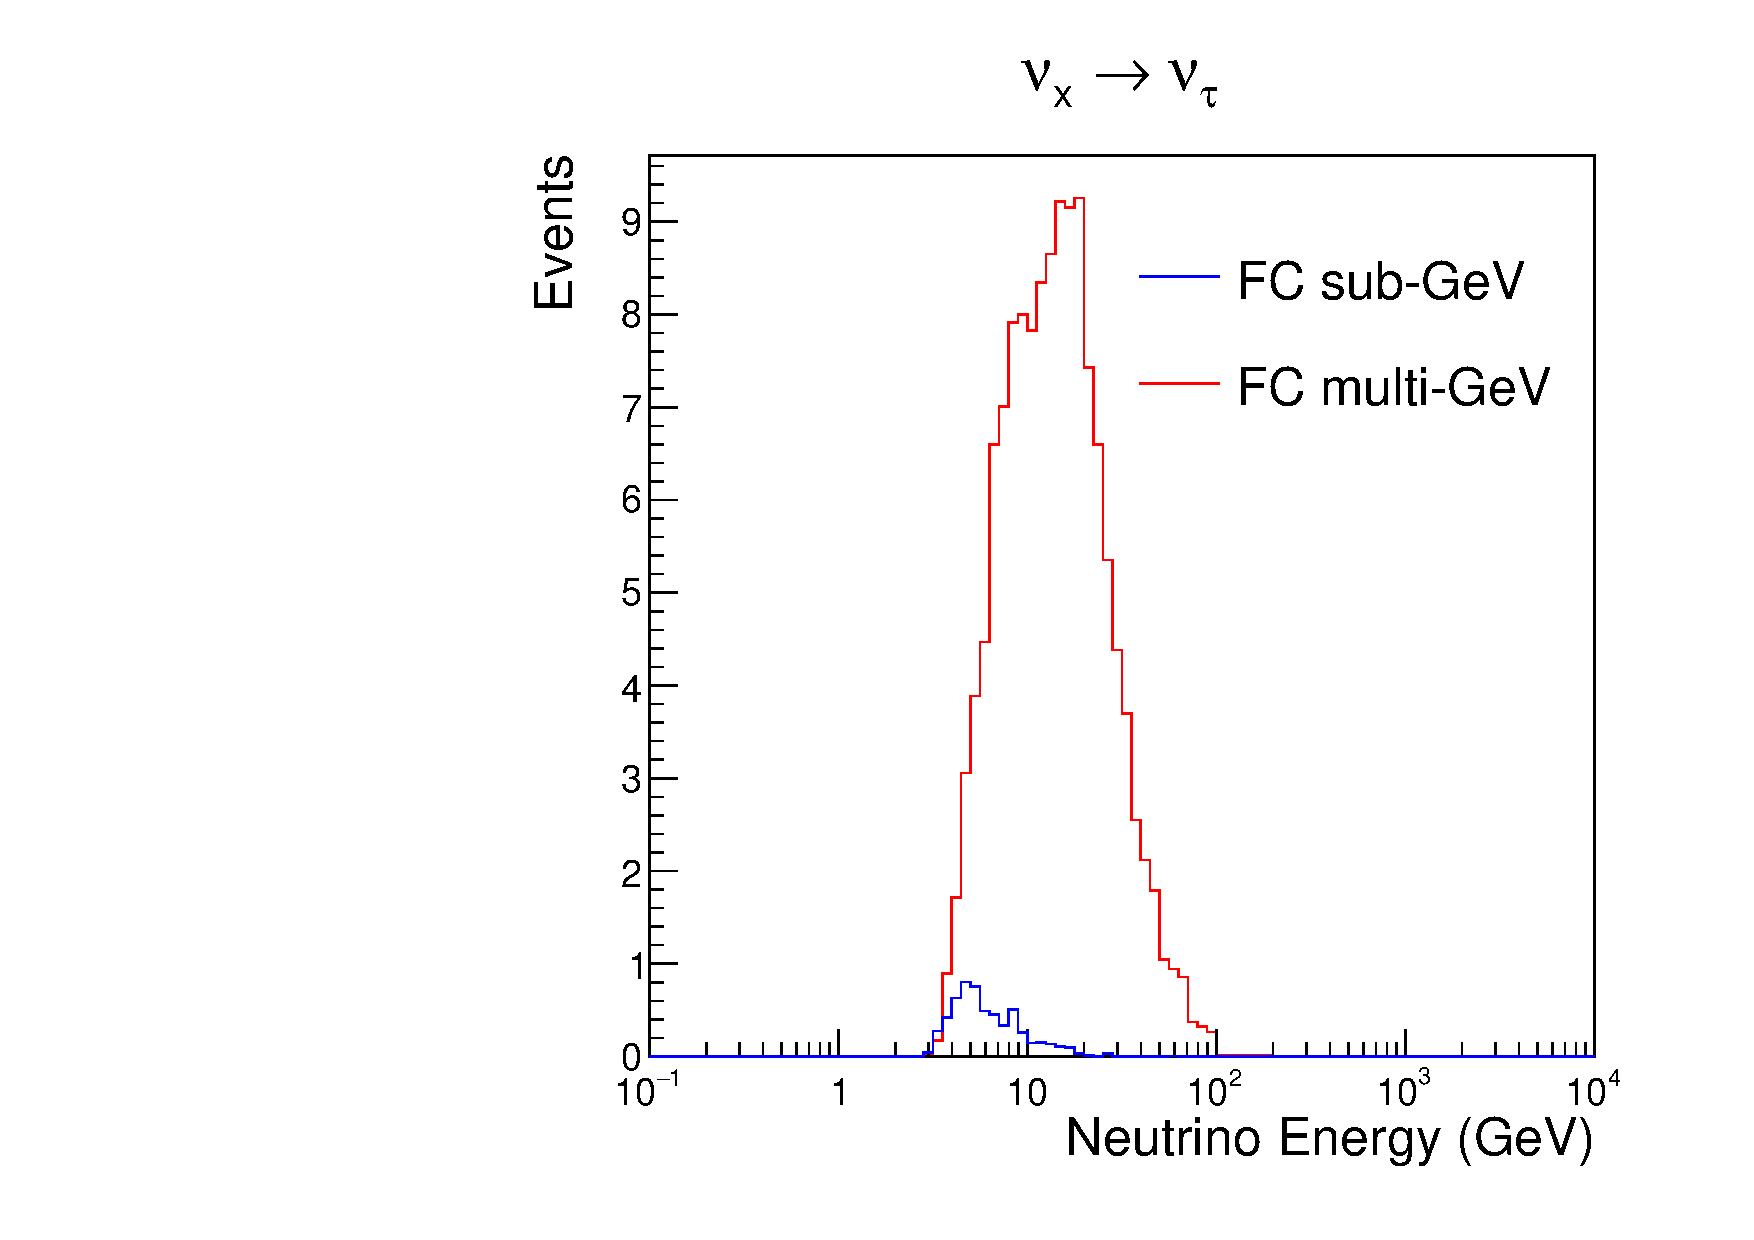
\includegraphics[width=\textwidth, trim={0mm 0mm 0mm 0mm}, clip,page=1]{Figures/Simulations/NeutrinoEnergyDist_NuTau.pdf}
  \end{subfigure}%
  \caption{The predicted neutrino flux of the fully contained (FC) sub-GeV and multi-GeV, partially contained (PC), and upward-going muon (\quickmath{\text{Up-}\mu}) events. The prediction is broken down by the \quickmath{\nu_{x} \rightarrow \nu_{e}} prediction (top left), \quickmath{\nu_{x} \rightarrow \nu_{\mu}} prediction (top right) and \quickmath{\nu_{x} \rightarrow \nu_{\tau}} prediction (bottom). \quickmath{\nu_{x}} represents the flavours of neutrinos produced in the cosmic ray showers (electron and muon). Asimov A oscillation parameters are assumed (given in \autoref{tab:Theory_ParameterSets}).}
  \label{fig:Simulations_NeutrinoEnergyDistribution}
\end{figure}

The first two steps in the FC reconstruction remove the majority of cosmic ray muons by requiring a significant amount of ID activity compared to that measured in the OD. Events that pass this cut are typically very high momentum muons or events that leave very little activity in the OD. Consequently, a third reduction step is then applied to select cosmic-ray muons that pass the initial reduction step. A purpose-built cosmic muon fitter is used to determine the entrance (or exit) position of the muon and a cut is applied to OD activity contained within \quickmath{8\text{m}} of this position. Flasher events are removed in the fourth reduction step which is based on the close proximity of PMT hits surrounding the PMT producing the flash. Events that pass all these reduction steps are reconstructed with the \texttt{APFit} algorithm. The fifth step of the reduction uses information from the more precise fitter to repeat the previous two steps with tighter cuts. Muons below the Cherenkov threshold can not generate optical photons in the ID but the associated decay electron can due to its lower mass. These are the types of events targeted in the fifth reduction step. The final cuts require the event vertex to be within the fiducial volume (\quickmath{0.5\text{m}} from the wall although the nominal distance is \quickmath{2.0\text{m}}), visible energy \quickmath{E_{vis} > 30\text{MeV}} and fewer than 16 hits within the higher energy OD cluster. The culmination of the fully contained reduction results in \quickmath{8.09} events/day in the nominal fiducial volume \cite{thesis_miao}. The uncertainty in the reconstruction is calculated by comparing Monte Carlo prediction to data. The largest discrepancy is found to be \quickmath{1.3\%} in the fourth reduction step.

The PC and \quickmath{\text{Up-}\mu} events are processed through their own reduction processes detailed in \cite{Ashie_2005}. Both of these samples are reconstructed with the \texttt{APFit} algorithm rather than \texttt{fiTQun}. This is because the efficiency of reconstructing events that leave the detector has not been sufficiently studied for reliable systematic uncertainties with \texttt{fiTQun}. The PC and \quickmath{\text{Up-}\mu} samples acquire events at approximately \quickmath{0.66} and \quickmath{1.44} events/day.

Beam neutrinos events undergo the same reduction steps as FC events and are then subject to further cuts \cite{t2k_tn_027}. The GPS system that links the timing between the beam facility and SK needs to be operating correctly and there should be no activity within the detector in the previous \quickmath{100 \mu\text{s}} before the trigger. The events then need to triggered between \quickmath{-2 \mu\text{s}} and \quickmath{10\mu\text{s}} of the expected spill timing.

The beam neutrino samples are not split by visible energy since their energy range is smaller than the atmospheric neutrino events. Following the T2K analysis in \cite{Dunne2020-uf}, only single-ring beam neutrino events are considered. Similar to atmospheric event selection, the number of decay electrons is used as a proxy for distinguishing CCQE and CCRES events. The expected neutrino energy, broken down by the number of decay electrons, is given in \autoref{fig:Simulations_NeutrinoEnergyDistribution_T2K}.

\begin{figure}[h]
  \begin{subfigure}[t]{0.49\textwidth}
    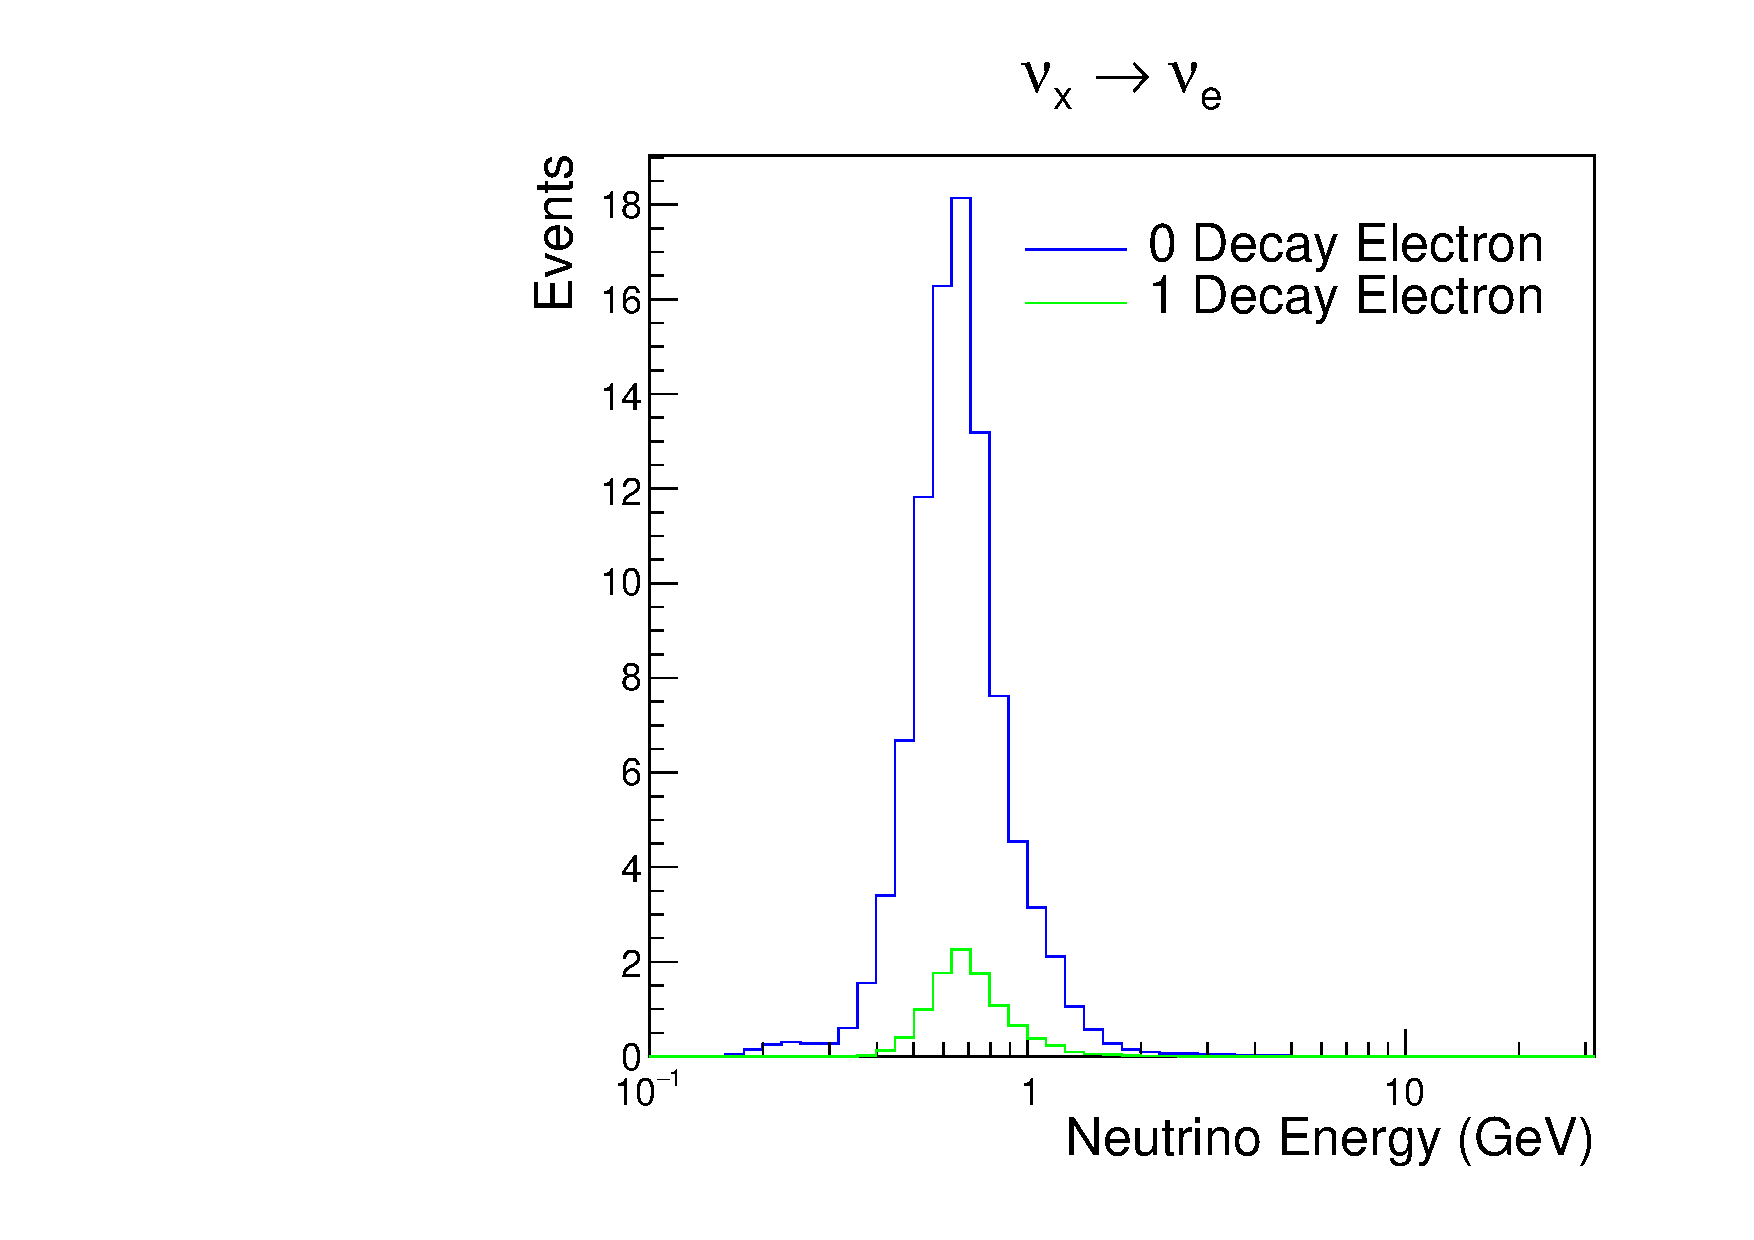
\includegraphics[width=\textwidth, trim={0mm 0mm 0mm 0mm}, clip,page=1]{Figures/Simulations/NeutrinoEnergyDist_T2K_NuE.pdf}
  \end{subfigure}%                                                                                                                                                                                         
  \begin{subfigure}[t]{0.49\textwidth}
    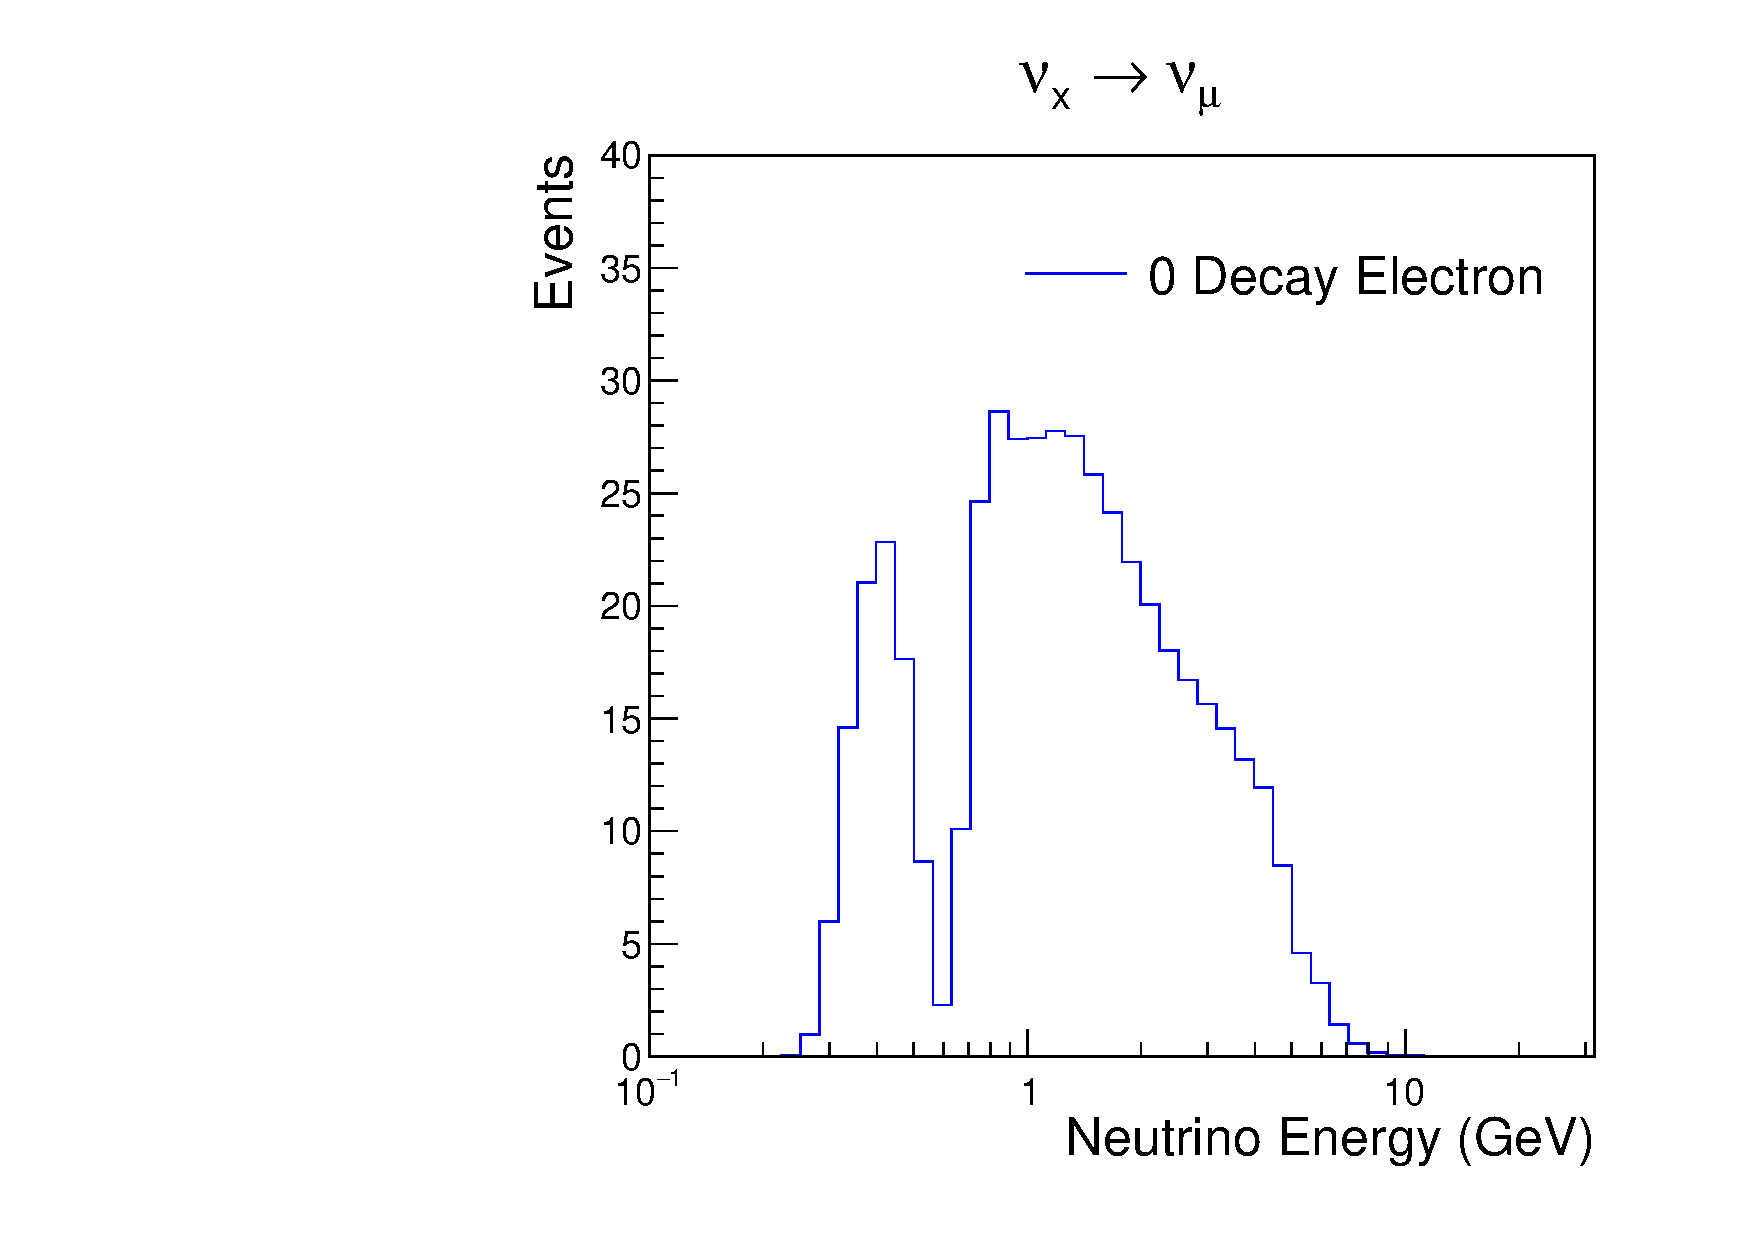
\includegraphics[width=\textwidth, trim={0mm 0mm 0mm 0mm}, clip,page=1]{Figures/Simulations/NeutrinoEnergyDist_T2K_NuMu.pdf}
  \end{subfigure}
  \caption{The predicted flux of beam neutrinos, as a function of neutrino energy. The predictions are broken down by the number of decay electrons associated with the particular events. Asimov A oscillation parameters are assumed (given in \autoref{tab:Theory_ParameterSets}).}
  \label{fig:Simulations_NeutrinoEnergyDistribution_T2K}
\end{figure}
